\documentclass[12pt]{article}
\usepackage[utf8]{inputenc}
\usepackage[spanish,es-tabla]{babel}
\usepackage[square,sort,comma,numbers]{natbib}
\usepackage{amssymb,amsmath,amsthm,amsfonts}
\usepackage{calc}
\usepackage{afterpage}
\usepackage{gensymb}
\usepackage{natbib}
\usepackage{url}
\usepackage{amsmath}
\usepackage{graphicx}
\usepackage{parskip}
\usepackage{fancyhdr}
\usepackage{vmargin}
\usepackage[table,xcdraw]{xcolor}
\usepackage[top=2cm,bottom=2cm]{geometry}
\usepackage{graphicx}
\usepackage{pdflscape}
\usepackage{multirow}
\usepackage{caption}
%\usepackage{subfigure}
\usepackage{xurl}
\usepackage{booktabs}
\usepackage{subfig}
\usepackage{float}
\usepackage{listings}

%Agregados
\usepackage[shortlabels]{enumitem}

\def\BibTeX{{\rm B\kern-.05em{\sc i\kern-.025em b}\kern-.08em
    T\kern-.1667em\lower.7ex\hbox{E}\kern-.125emX}}
\setmarginsrb{3 cm}{2.5 cm}{3 cm}{2.5 cm}{1 cm}{1.5 cm}{1 cm}{1.5 cm}

\title{Ejercicio N$^{\circ}$1}					 % Titulo
\author{Elias Obreque \\ Gustavo Ceballo \\ Maibeth Sánchez}					 % Autor
\date{\today}						% Fecha


\makeatletter
\let\thetitle\@title
\let\theauthor\@author
\let\thedate\@date
\makeatother

\pagestyle{fancy}
\fancyhf{}
\lhead{\thetitle}
\cfoot{\thepage}

\begin{document}

%%%%%%%%%%%%%%%%%%%%%%%%%%%%%%%%%%%%%%%%%%%%%%%%%%%%%%%%%%%%%%%%%%%%%%%%%%%%%%%%%%%%%%%%%

\begin{titlepage}
	\centering
    \vspace*{0.0 cm}
    
\includegraphics[scale = 0.13]{Logo_Uchile_modern.png}\\[1.0 cm]	% Logo Universidad
    \textsc{\LARGE Universidad de Chile}\\[2.0 cm]	% Nombre Universidad
	\textsc{\Large EL7012}\\[0.5 cm]				 % Codigo Curso
	\textsc{\large Control Inteligente de Sistemas, Otoño}\\[0.2 cm]		 % Nombre Curso
	\rule{\linewidth}{0.2 mm} \\[0.2 cm]
	{ \huge \bfseries \thetitle}\\
	\rule{\linewidth}{0.2 mm} \\[0.5 cm]
	
	\begin{minipage}{0.4\textwidth}
		\begin{center} \large
			\emph{Autor:}\\
			\theauthor\linebreak
			\end{center}
	\end{minipage}\\[1.5 cm]
	
	{\large \thedate}\\[1.5 cm]

	\vfill
	
\end{titlepage}

%%%%%%%%%%%%%%%%%%%%%%%%%%%%%%%%%%%%%%%%%%%%%%%%%%%%%%%%%%%%%%%%%%%%%%%%%%%%%%%%%%%%%%%%%

\tableofcontents
\listoffigures
\listoftables
\afterpage{\null\newpage}
\newpage
\thispagestyle{empty}
\pagebreak
\newpage
\setcounter{page}{1}

%%%%%%%%%%%%%%%%%%%%%%%%%%%%%%%%%%%%%%%%%%%%%%%%%%%%%%%%%%%%%%%%%%%%%%%%%%%%%%%%%%%%%%%%%

\section{Introducción}

La  mayoría  de  los  sistemas  tienen  un  comportamiento  no  lineal,  excepto  en  un determinado rango de operación donde pueden ser considerados lineales. En ocasiones un modelo lineal es insuficiente para explicar un fenómeno por lo que se debe recurrir a Modelos No Lineales.

Los modelos basados en redes neuronales y sistemas difusos han sido empleados para la identificación, dado que han mostrado una grancapacidad para aproximar funciones no lineales desconocidas, además de que ofrecen una estructura general tan compleja o sencilla como el problema lo demande. Por un lado, las redes neuronales son estructuras matemáticas inspiradas en las estructuras biológicas compuestas por neuronas, en donde a través de elementos relativamente simples (llamados neuronas)que efectúan operaciones y procesos muy sencillos logran, mediante interconexiones, realizar procesos complejos y procesamiento de información en paralelo. En general se consideran redes neuronales conformadas por “capas” de neuronas, donde una capa procesa la información recibida en paralelo y la envía a la siguiente capa de neuronas. Por otro lado, los sistemas difusos son también estructuras matemáticas, aunque estos se encuentran inspirados en los procesos de pensamiento y toma de decisiones llevados a cabo por los humanos, así como en la teoría de conjuntos difusos propuesta por Lofti Zadeh.

En este ejercicio se dará solución al Problema 1.


\subsection{Problema 1}

Considere la siguiente serie no lineal dinámica:

\begin{align}
y(k)= (0.8 - 0.5 exp\{-y^2(k- 1)\})y(k - 1)\nonumber \\
-(0.3 + 0.9 exp\{-y^2(k - 1)\})y(k - 2)\nonumber \\
+u(k - 1) + 0.2u(k - 2) + 0.1u(k - 1)u(k - 2) + e(k)
\label{e_serie}
\end{align}

donde el ruido del sistema

\begin{equation}
e(k)=  0.5 exp\{-y^2(k- 1)\}\beta(k)
\label{e_error}
\end{equation}

depende del estado previo de la salida del modelo, y $\beta(k)$ es un ruido blanco.

Como usted sabe existen varias técnicas que se pueden emplear para la modelación a partir de estos datos, por lo que debe seleccionar el tipo de modelo más adecuado para este tipo de sistema. Para este trabajo se le pide detallar la metodología utilizada para:

\begin{enumerate}[a)]
\item Generar 600 datos a partir de esta serie. Considere 55\% para entrenamiento, 25\% test y 20\% validación.
\item Obtener un modelo de predicción lineal, difuso tipo-1 (T\&S) y neuronal para la salida. Evaluar las predicciones a 1, 8 y 16 pasos. Comparar el desempeño de todos los modelos a partir de las métricas más apropiadas tales como RMSE, MAPE, MAE, entre otras. Comente.
\item Construir el intervalo de predicción de los modelos obtenidos en b) utilizando el método de la covarianza.
\item Evaluar los intervalos de predicción obtenidos en b) realizando predicciones a 1, 8, y 16 pasos. Comparar el desempeño de los modelos a partir de las métricas más apropiadas tales como ancho del intervalo, probabilidad de cobertura, entre otras.
\item Construir el intervalo de predicción del modelo difuso encontrado en a) con el método de optimización min-max. Compare este intervalo de predicción con el intervalo obtenido utilizando el método de la covarianza. Comente.
\item Construir el intervalo de predicción neural utilizando el método de Joint Supervision. Compare con los métodos anteriores.
\item Seleccione el modelo más apropiado y justifique.
\end{enumerate}

\newpage
\section{Generación de Datos}

En esta estapa es necesario generar datos que representen la dinámica del sistema en la mayor cantidad de rangos de operación posibles, ya que el modelo obtenido tiene un ancho de banda acotado, y por lo tanto las dinámicas definidas por fuera de dicha banda podrían no ser representadas adecuadamente. Para lo cual se debe diseñar una entrada $u(k)$ que excite a la planta en el rango de frecuencias en que se encuentran los fenómenos de interés.

En este trabajo se propone el uso de señales binarias pseudo aleatorias (Pseudo Random Binary Signal, PRBS),  ya  que  es  una  de  las  señales  más  utilizadas  en  identificación  de sistemas. Esta es una señal periódica, determinística y que  posee  principalmente  propiedades  similares  al  ruido  blanco  (contenido  muy  rico  en frecuencias) \citep{nelles2013nonlinear}.

Para generar la señal se suponen los siguientes parámetros de interés $f_{min}=0.2 Hz$, $f_{max}=1 Hz$ y tiempo de muestreo $T_S=0.01$. Con los parámetros anteriores, y utilizando la expresión

\begin{equation}
n=\frac{log(f_c/f_{min}+1)}{log(2)})
\label{e_}
\end{equation}

con $f_c=2.5*f_{max}=2.5 Hz$, se genera una PRBS de orden $n= 4$, por lo que el largo máximo corresponde a $N = 2^n - 1 = 15$. A su vez, la cantidad de muestras por bit son $N_{s} = 40$,  lo cual supera el número de iteraciones en el que sistema se establece ante una entrada escalón sin ruido aproximadamente 20 iteraciones, por lo que la PRBS debe ser replicada 400 veces con diferentes condiciones iniciales para obtener los 6000 datos de interés. Finalmente se genera la APRBS variando la amplitud aleatoriamente de la PRBS generada, Fig.\ref{f_APRBS} y se aplica a la serie no lineal como se muestra en la Fig.\ref{f_SerieNoLineal}.

\begin{figure}
\centering
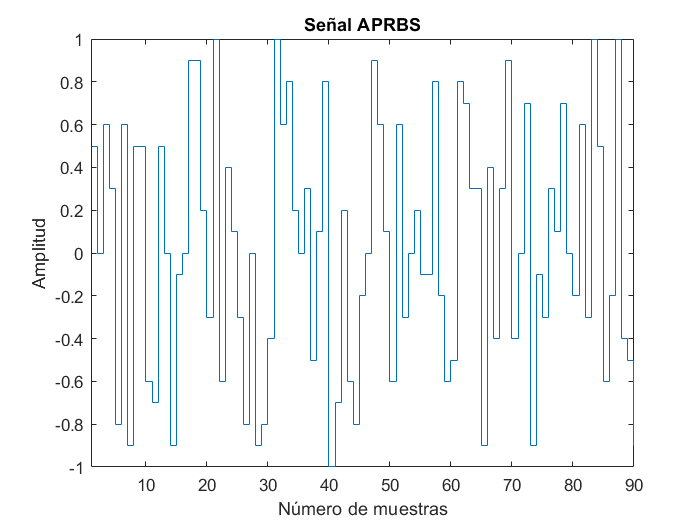
\includegraphics[width=10cm,height=7cm]{imag/APRBS}
\caption{Señal APRBS con Amplitud entre -1 y +1.}
\label{f_APRBS}
\end{figure}

\begin{figure}
\centering
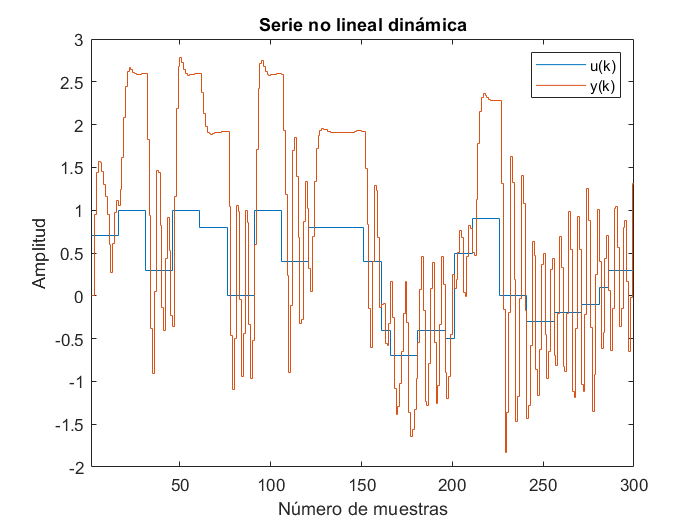
\includegraphics[width=10cm,height=7cm]{imag/SerieNoLineal}
\caption{Respuesta de la serie no lineal.}
\label{f_SerieNoLineal}
\end{figure}


Una vez obtenidos los datos experimentales de entrada-salida, éstos son clasificados en tres conjuntos con distinta información: datos de entrenamiento, datos
de validación y datos de prueba; esto con el fin de evaluar adecuadamente los modelos
generados. El conjunto de entrenamiento se utiliza para determinar los parámetros del
modelo. El conjunto de prueba permite comparar distintas estructuras de los modelos
generados. Finalmente, el conjunto de validación permite verificar el sobreajuste del
modelo óptimo obtenido, evaluándolo en un nuevo conjunto de datos (distintos a los
datos del conjunto de entrenamiento y prueba), analizando su capacidad de
generalización. En este caso se utiliza una división de 55\% de los datos para entrenamiento, 25\% para prueba y 20\% validación.

\section{Modelos de predicción}
\subsection{Modelo lineal}

En este caso, supondremos que se ajustará un modelo lineal suponiendo que el sistema real es lineal con ruido blanco gaussiano aditivo, es decir,


\begin{equation}
y(k)=a_1 y(k-1)+a_2 y(k-2)+b_1 u(k-1)+b_2 u(k-2)+e(k)
\label{e_ModeloLineal}
\end{equation}

Luego, se propone un modelo lineal para llevar a cabo la predicción a 1 paso, de modo tal que:
Predicción a 1 paso:

\begin{equation}
\hat{y}(k)=\hat{a}_1 y(k-1)+\hat{a}_2 y(k-2)+\hat{b}_1 u(k-1)+\hat{b}_2 u(k-2)
\label{e_Pre1paso}
\end{equation}

Este modelo no considera un valor constante o bias dao el supuesto que el sistema es lineal con ruido blanco aditivo. En caso que se sospechara que existe un bias o tendencia (trend) en el sistema, se puede agregar otro vector de unos a la matriz de regresores (o matriz de información). Para llevar a cabo la estimación de los parámetros del modelo se utilizó la técnica de mínimos cuadrados, es decir:

\begin{equation}
\hat{\theta}=(Xent^T*Xent)^{-1}*Xent^T*\hat{y}(k)
\label{e_AjustMinCuadrados}
\end{equation}


En que $\hat{\theta}=[\hat{a}_1 \quad \hat{a}_2 \quad \hat{b}_1 \quad \hat{b}_2]^T$ es el vector de parámetros y $Xent$ es la matriz de regresores con los valores de las $n$ muestras ordenados por filas.

Los valores que se obtuvieron de los parámetros fueron los siguientes:


\begin{equation}
\hat{\theta}=\left(
                \begin{array}{c}
                  \hat{a}_1  \\
                  \hat{a}_2  \\
                  \hat{b}_1  \\
                  \hat{b}_2  \\
                \end{array}
              \right)
=\left(
   \begin{array}{c}
     0.8601 \\
     -0.6930 \\
     0.9724 \\
     0.3486 \\
   \end{array}
 \right)
\label{e_ValoresCoeficientes}
\end{equation}

En la Fig. \ref{f_G123}, se muestran las gráficas de la predicción a un paso en cada conjunto de datos, a saber, conjunto de entrenamiento, prueba y validación. Esto es solo a modo de comparación puesto que finalmente, lo relevante de nuestro modelo, es el comportamiento o bondad de ajuste en el conjunto de validación. Evidentemente que los datos de los parámetros usados en las predicciones, para todos los conjuntos, son aquellos obtenidos con el conjunto de entrenamiento, sin embargo, la matriz de represores y salidas cambian dependiendo del conjunto que se esté usando para predicción. A continuación, en la Tabla \ref{t_NoLinealp1}, se presentan las métricas de bondad del ajuste o errores en los diversos conjuntos de datos, a saber, conjunto de datos de entrenamiento, prueba o test y validación.

\begin{figure}
		\centering
		\captionsetup{justification=centering}
		\subfloat[Predicción a 1 paso en conjunto de entrenamiento]{
		 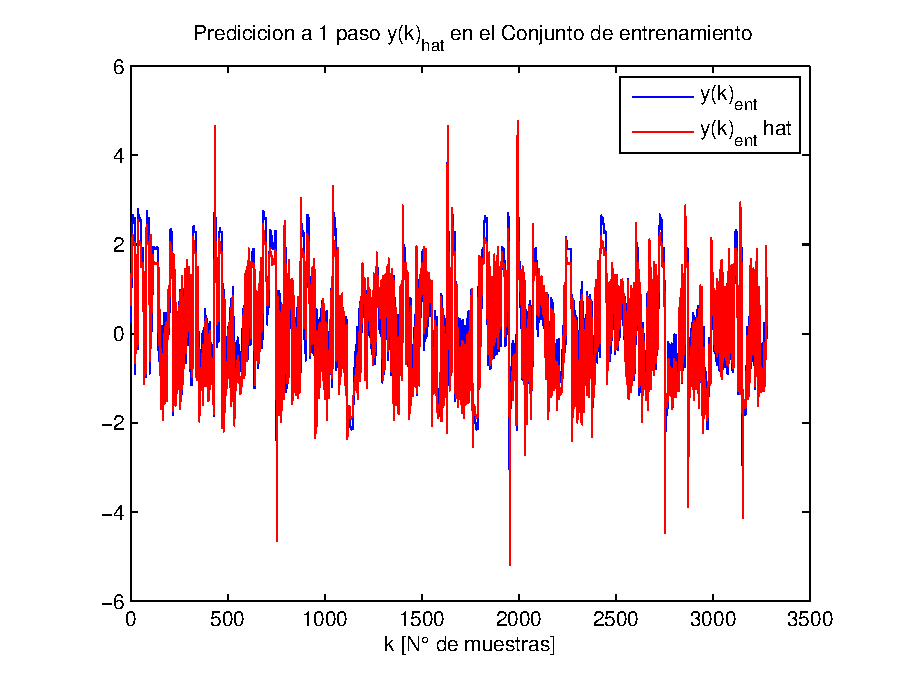
\includegraphics[width=0.5\textwidth]{imag/Figura_1}}\\
		\subfloat[Predicción a 1 paso en conjunto de prueba]{
		 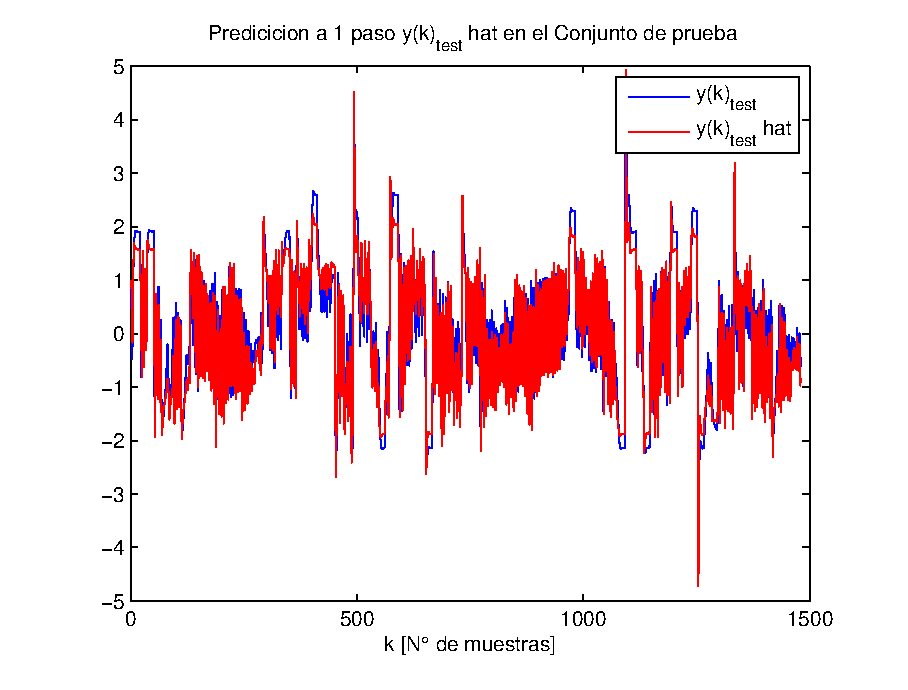
\includegraphics[width=0.5\textwidth]{imag/Figura_2}}
		\subfloat[Predicción a 1 paso en conjunto de validación]{
		 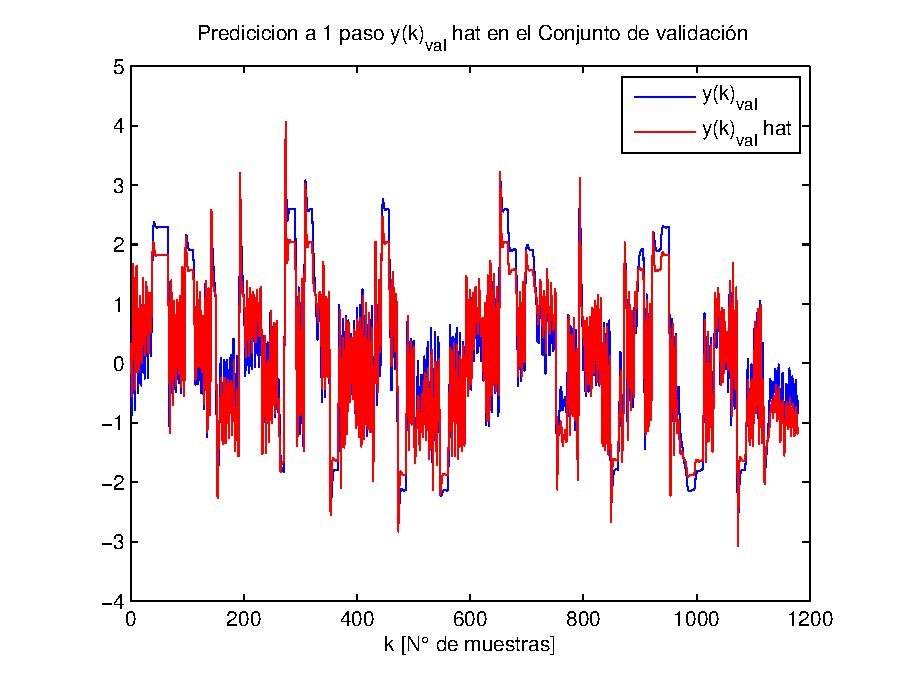
\includegraphics[width=0.5\textwidth]{imag/Figura_3}}\\
		\caption{Predicción del modelo Lineal.}
		\label{f_G123}
\end{figure}

% Table generated by Excel2LaTeX from sheet 'Sheet1'
\begin{table}[h!]
  \centering
  \caption{Errores o Métricas de bondad de ajuste a 1 paso}
\begin{tabular}{|l|l|l|l|}
	\hline
	Métricas & Conjunto Entrenamiento & Conjunto prueba & Conjunto validación \\ \hline
	RMSE     & 0.0869                 & 0.0559          & 0.0954              \\ \hline
	MAPE     & 162.2793               & 220.0863        & 238.2150            \\ \hline
	MAE      & 0.3569                 & 0.3465          & 0.6020              \\ \hline
\end{tabular}
  \label{t_NoLinealp1}%
\end{table}%

Es interesante notar que los ajustes del modelo, en todos los conjuntos, son bastante comparables entre sí, es decir, en general, los errores son similares en cuanto a RMSE y MAE. Esto también se puede apreciar al observar la Fig. \ref{f_G123} respectivamente. Si bien, el conjunto de entrenamiento presenta el menor MAPE, a su vez, el conjunto de entrenamiento, presenta el menor RMSE.

\subsubsection{Predicciones a 1, 8, y 16
	pasos}

Para efectos de apreciar la robustez de este modelo, llevaremos a cabo la predicción a 8 y 16 pasos respectivamente, en el conjunto de validación del modelo lineal, para luego compararlos con los demás modelos, a saber, modelo de Takagi y Sugeno y Modelo Neuronal para el mismo conjunto de validación, Fig. \ref{f_G456}.
\begin{figure}[h!]
		\centering
		\captionsetup{justification=centering}
		\subfloat[Predicción a 1 paso en el conjunto de validación para el Modelo Lineal]{
		 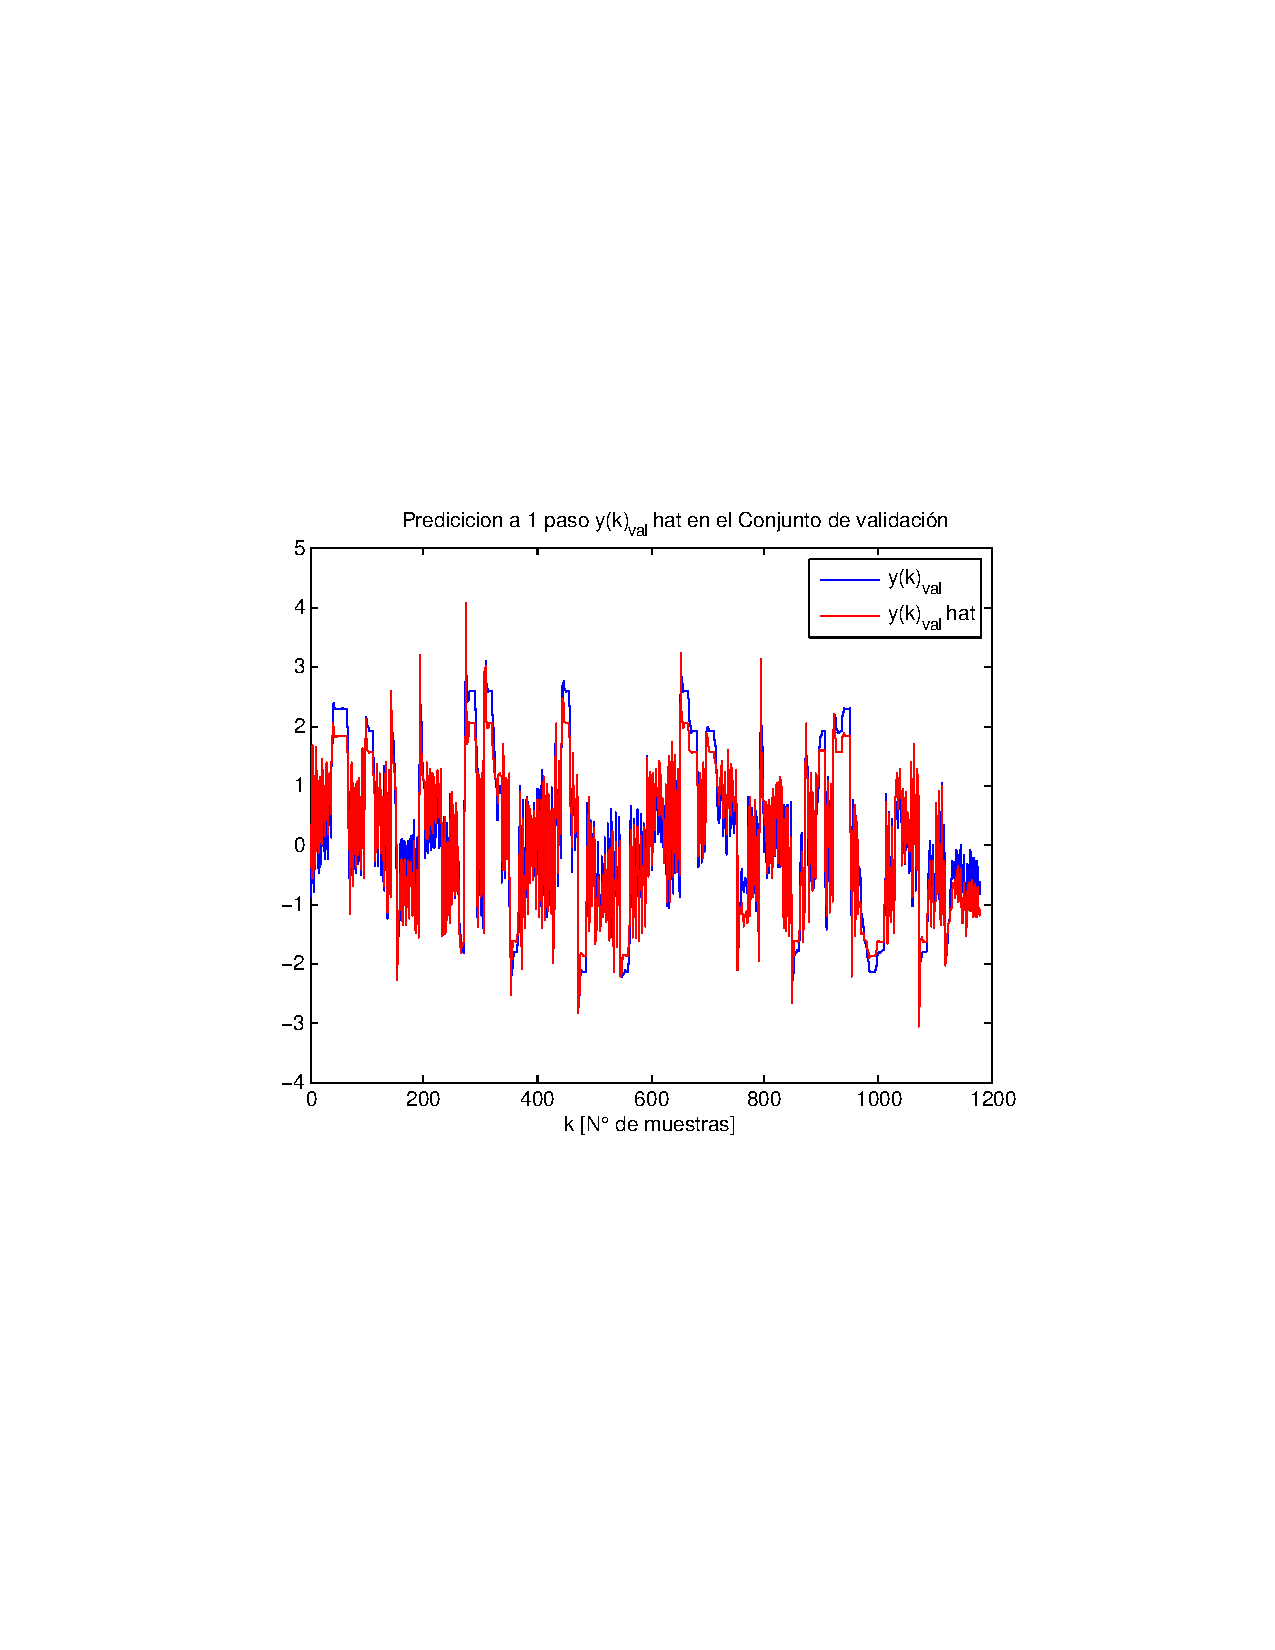
\includegraphics[width=0.5\textwidth]{imag/Figura_4}}\\
		\subfloat[Predicción a 8 pasos en el conjunto de validación para el Modelo Lineal.]{
		 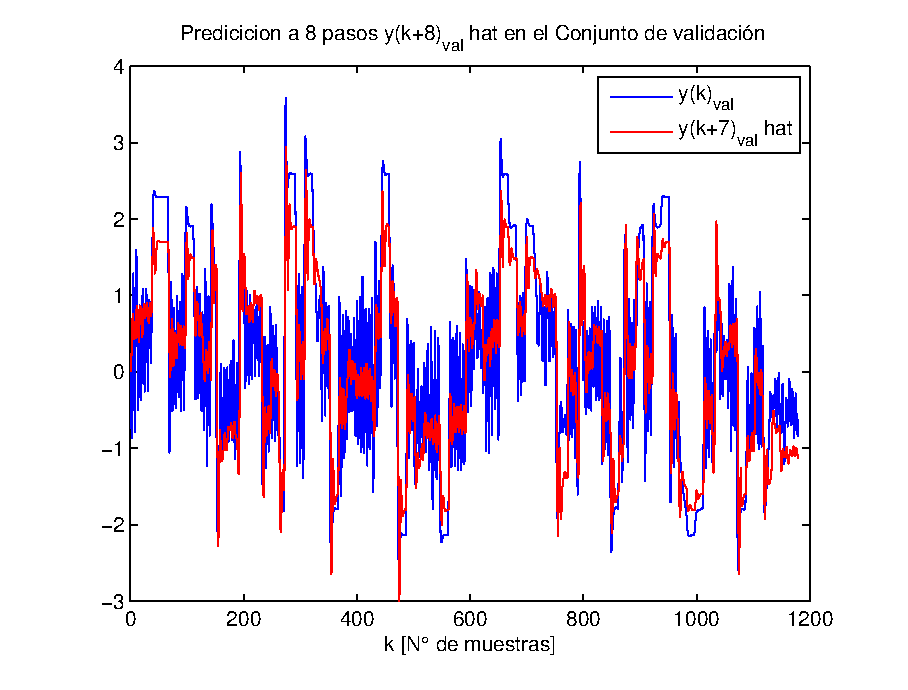
\includegraphics[width=0.5\textwidth]{imag/Figura_5}}
		\subfloat[Predicción a 16 pasos en el conjunto de validación para el Modelo Lineal.]{
		 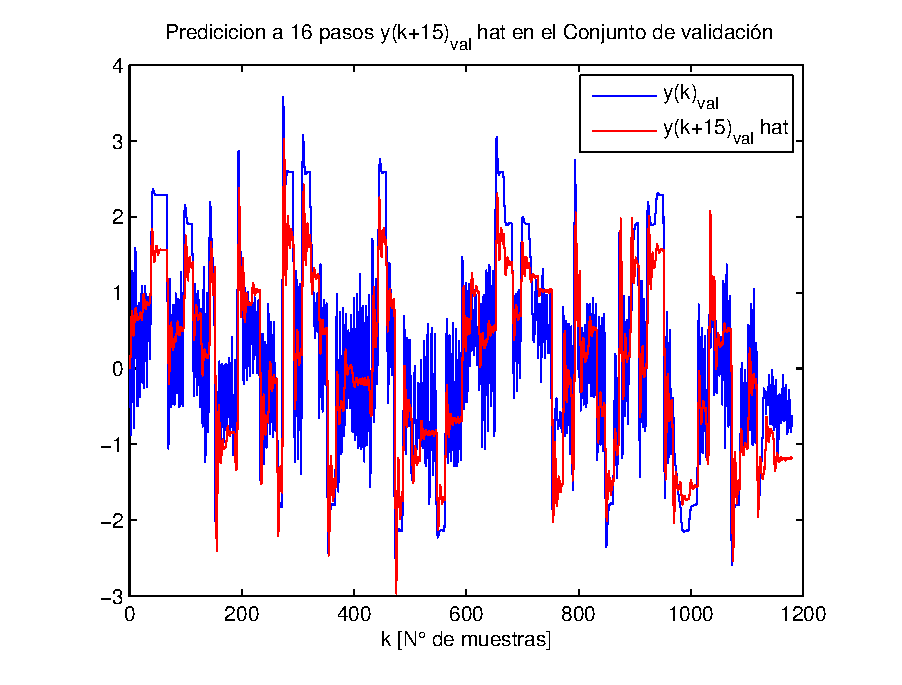
\includegraphics[width=0.5\textwidth]{imag/Figura_6}}\\
		\caption{Predicción del modelo Lineal.}
		\label{f_G456}
\end{figure}

\clearpage
\newpage
\subsubsection{Intervalos de predicción}
En este caso, se pueden definir 2 modelos adicionales que den cuenta de un intervalo que contenga un porcentaje de las muestras al interior del mismo. A saber, podríamos determinar un modelo por arriba ($y_u$) y uno por abajo ($y_l$) del modelo de valor esperado $y_{val}$, con los datos del conjunto de validación, determinado en la sección anterior.

Estos modelos se podrían construir considerando la adición de la varianza de las salidas del conjunto de validación entre el valor real y el estimado, es decir, el intervalo tendría la siguiente expresión para ambos modelos:

\begin{equation}
\hat{y}_u(k)=X_{val}(k)\hat{\theta}(k)+\alpha[Var(y(k)_{val}-\hat{y}_{val}(k))]^{1/2}
\label{e_MLocal_G}
\end{equation}

\begin{equation}
\hat{y}_u(k)=X_{val}(k)\hat{\theta}(k)-\alpha[Var(y(k)_{val}-\hat{y}_{val}(k))]^{1/2}
\label{e_MLocal2_G}
\end{equation}

En que $\alpha$ es un parámetro de ajuste que tiene relación con el porcentaje de cobertura que tendría el intervalo, Var() es el operador varianza de las salidas reales y estimadas en el conjunto de validación y $X_{val}(k)\hat{\theta}(k)$ es el modelo obtenido de valor esperado visto en la sección anterior, es decir,
\begin{equation}
\hat{y}_{val}(k)=X_{val}(k)\hat{\theta}(k)
\end{equation}

Así entonces, podemos determinar los modelos por arriba y por abajo del modelo clásico de valor esperado, los cuales nos definen el intervalo. En la Fig. \ref{f_G78}, se muestran las gráficas de las 3 curvas o modelos para la predicción a un paso con $\alpha=0,8$.

\begin{figure}[t!]
		\centering
		\captionsetup{justification=centering}
		\subfloat[Curvas para Intervalo del modelo lineal considerando predicción a 1 paso y $\alpha=0,8$]{
		 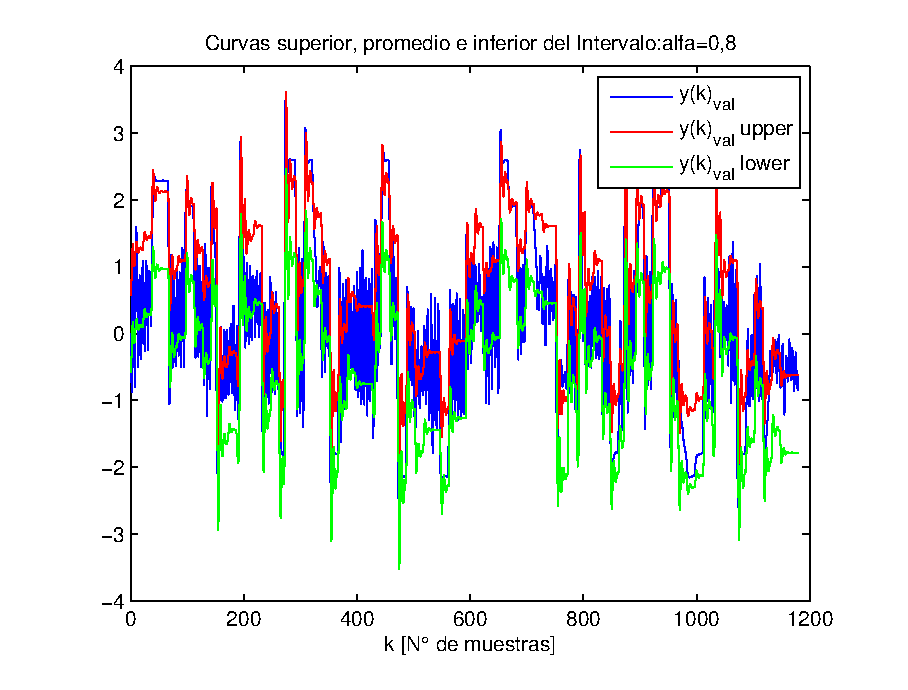
\includegraphics[width=0.5\textwidth]{imag/Figura_7}}
		\subfloat[Porción del gráfico]{
		 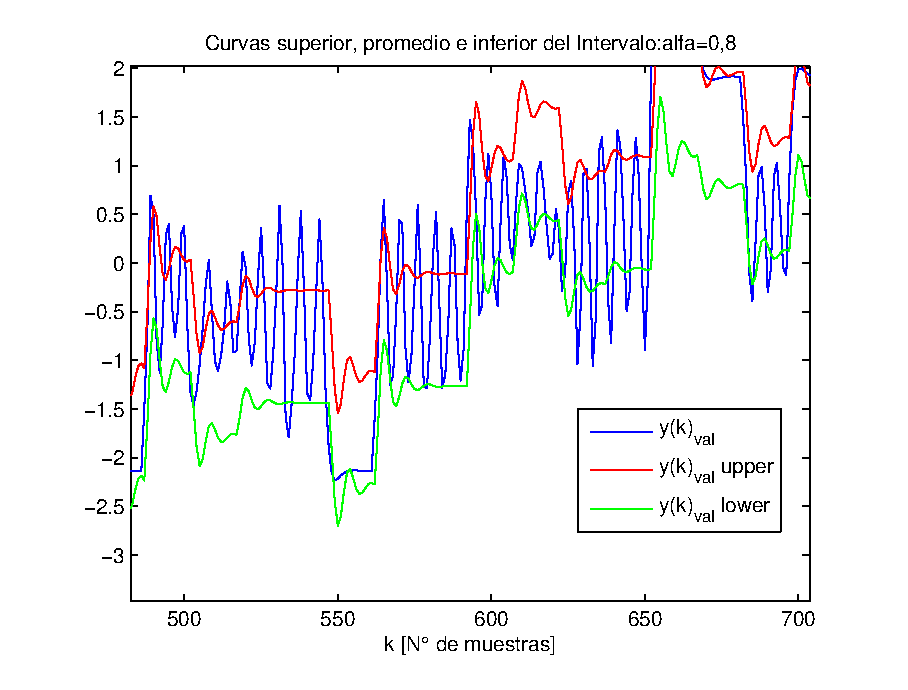
\includegraphics[width=0.5\textwidth]{imag/Figura_8}}\\
		\caption{Curvas para Intervalo del modelo lineal considerando predicción a 1 paso y $\alpha=0,8$}
		\label{f_G78}
\end{figure}

Ahora bien, podemos ir ajustando el valor de $\alpha$ para aumentar o disminuir el porcentaje de cobertura de las muestras de validación. En la Tabla \ref{t_G2}, se muestran las métricas PICP y PINAW las cuales miden el porcentaje de cobertura y ancho del intervalo respectivamente, para diferentes valores de $\alpha$ de la predicción a 1 paso. A modo de ejemplo, en la Fig. \ref{f_G910} se muestra el caso en que el parámetro $\alpha$ se aumenta a 1.5.
\begin{table}[h!]
	\centering
	\caption{Métricas de intervalo para diferentes valores de $\alpha$. }
	\begin{tabular}{|l|l|l|l|l|l|l|}
		\hline
		Parámetro $\alpha$ & 0,5&0,8&0,9&1&1,5&2\\
		\hline
		PICP (\%) & 32.2034 & 52.5424 & 58.7288 & 65.3390 & 885,593 & 96.1017 \\
		\hline
		PINAW & 11.687 & 18.6992 & 21.0366 & 23.7339 & 35.0609 & 46.7479 \\
		\hline
	\end{tabular}%
	\label{t_G2}%
\end{table}
\begin{figure}
		\centering
		\captionsetup{justification=centering}
		\subfloat[Curvas para Intervalo del modelo lineal considerando predicción a 1 paso y $\alpha=1.5$]{
		 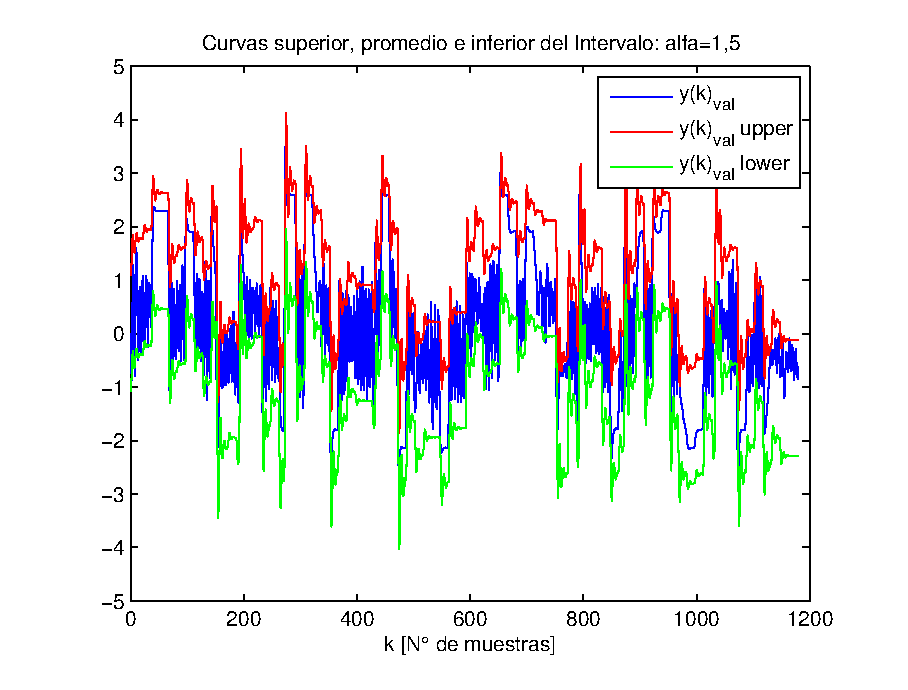
\includegraphics[width=0.5\textwidth]{imag/Figura_9}}
		\subfloat[Porción del gráfico]{
		 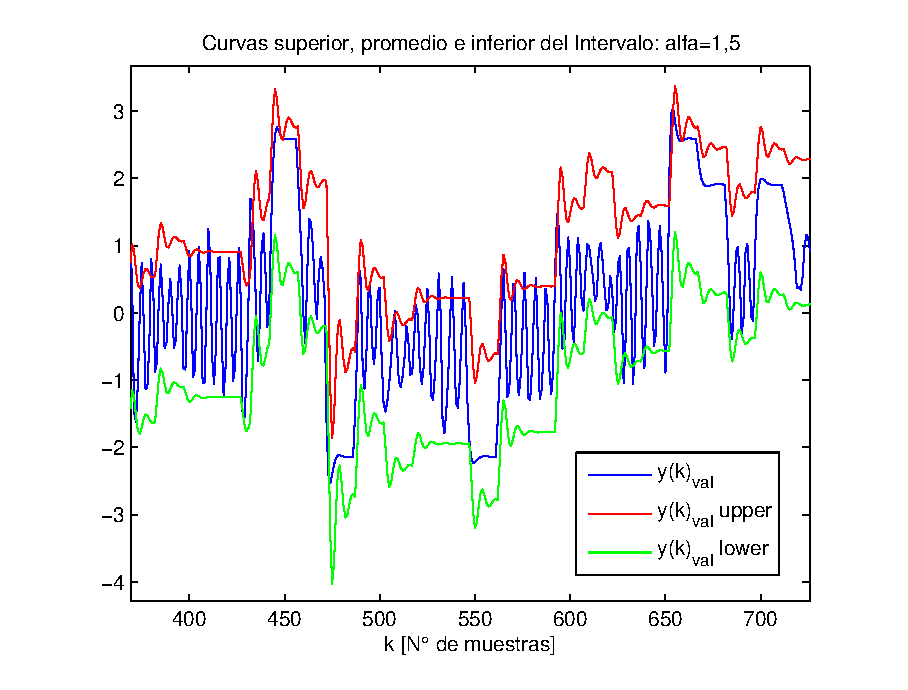
\includegraphics[width=0.5\textwidth]{imag/Figura_10}}\\
		\caption{Curvas para Intervalo del modelo lineal considerando predicción a 1 paso y $\alpha=1.5$}
		\label{f_G910}
\end{figure}
\clearpage
\newpage
Es evidente, que los datos de salida de la curva promedio (color azul) están casi completamente contenidos en el intervalo (entre curva de color rojo y verde respectivamente), de hecho, está en un 88,56\% contenida en el intervalo.
Ahora bien, en el caso de la construcción del intervalo de predicción a 8 y 16 pasos, se procede de manera análoga al caso de 1 paso, con la salvedad que se debe usar el modelo de 8 pasos y 16 pasos respectivamente.

A continuación, en la Fig. \ref{f_G1112}  se muestran los intervalos para el caso de 8 y 16 pasos considerando un parámetro $\alpha=0.8$, para efectos de comparación con el gráfico de la Fig. \ref{f_G78}.

\begin{figure}[h!]
		\centering
		\captionsetup{justification=centering}
		\subfloat[Curvas para Intervalo del modelo lineal considerando predicción a 8 pasos y $\alpha=0,8.$]{
		 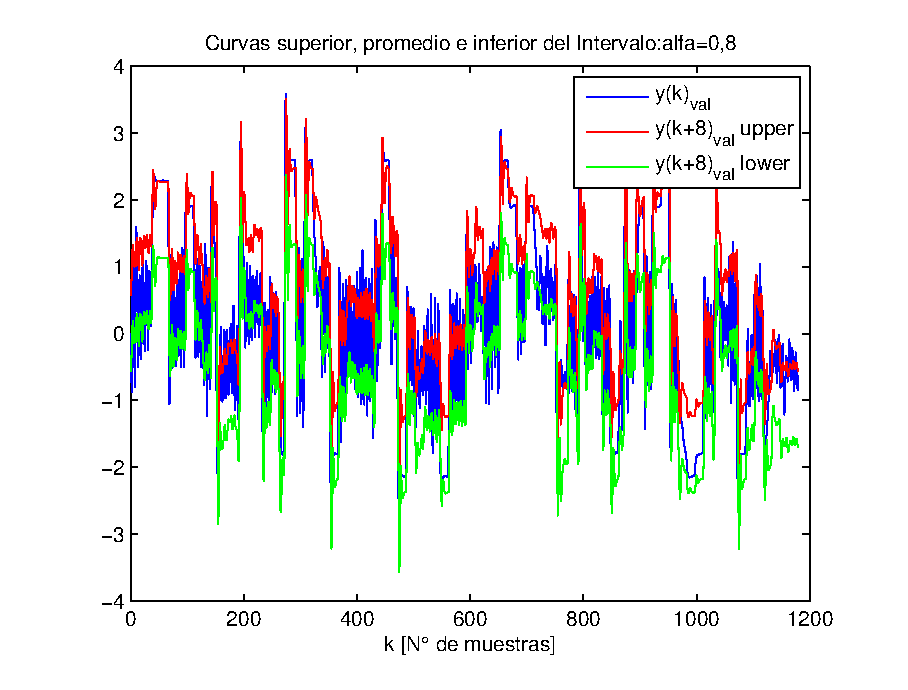
\includegraphics[width=0.5\textwidth]{imag/Figura_11}}
		\subfloat[Curvas para Intervalo del modelo lineal considerando predicción a 16 pasos y $\alpha=0,8.$]{
		 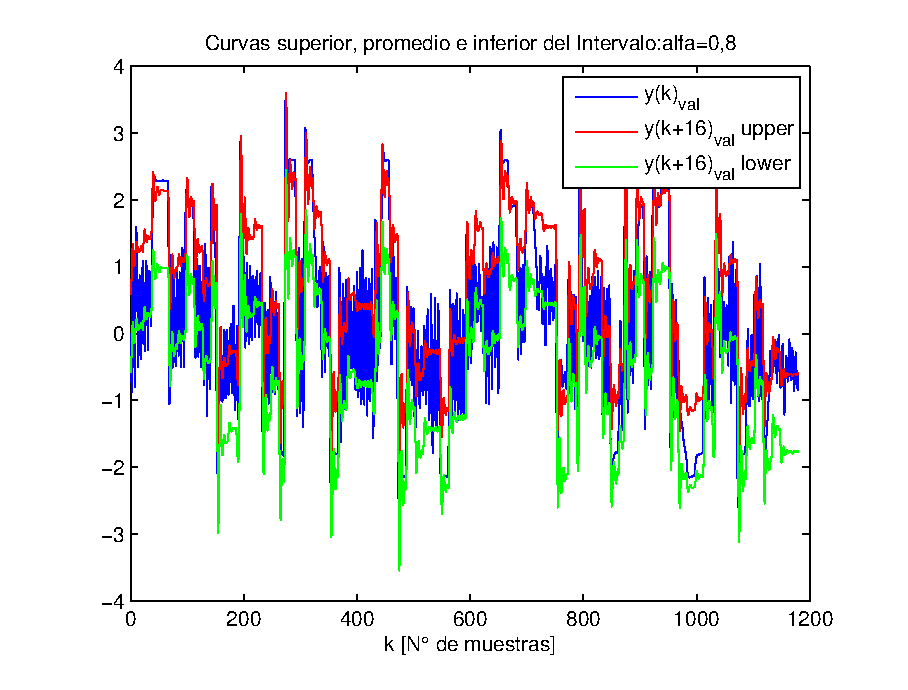
\includegraphics[width=0.5\textwidth]{imag/Figura_12}}\\
		\caption{Curvas para Intervalo del modelo lineal}
		\label{f_G1112}
\end{figure}

% Table generated by Excel2LaTeX from sheet 'Sheet1'
\begin{table}[htbp]
  \centering
  \captionsetup{justification=centering}
  \caption{Métricas de porcentaje de cobertura y ancho del intervalo para diferentes valores de $\alpha=0,8$ considerando intervalos de predicción a 1, 8 y 16 pasos respectivamente.}
\begin{tabular}{|l|l|l|l|}
	\hline
	Parámetro $\alpha=0,8$ & \multicolumn{3}{c|}{0.8}     \\ \hline
	& 1 pasos & 8 pasos & 16 pasos \\ \hline
	PICP (\%)              & 52.5424 & 52.7966 & 52.7966  \\ \hline
	PINAW                  & 18.6992 & 18.4244 & 18.7348  \\ \hline
\end{tabular}
  \label{t_G3}%
\end{table}%

Analizando las figuras anteriores y de la Tabla \ref{t_G3}, se puede concluir que las métricas de bondad para los intervalos son bastante similares. Por una parte, entendemos que esto se debe a que como el número de muestras del conjunto es muy elevado (1.200 muestras aproximadamente), respecto a las predicciones que se piden (1, 8 y 16 pasos), es más o menos evidente que no exista diferencia en los porcentajes de cobertura. La diferencia podría notarse en caso que los intervalos de predicción fueran a más muestras, por ejemplo, a 200 muestras en adelante.  Otro factor que favorece la similitud de las métricas anteriores, es el hecho que la entrada (señal APRBS) es bastante aleatoria y por tanto el ajuste no se ve más favorecido en un conjunto que en otro (conjunto de prueba o validación, por ejemplo).  Es decir, los parámetros de ajuste que se obtienen son similares, no importando que conjunto que usemos para entrenamiento.  Es evidente que el caso del conjunto de entrenamiento, lo favorece el hecho de que cuenta con más datos, pero dada la aleatoriedad de la señal de entrada, este factor no es tan incidente a la hora de comparar las métricas.

\newpage

\subsection{Modelo difuso Takagi-Sugeno Tipo-1}

Los modelos difusos de Takagi-Sugeno son estructuras basadas en la lógica difusa
que permiten representar procesos con dinámicas no lineales mediante la combinación
de información otorgada por modelos locales. Estos tipos de modelos pueden ser
expresados a partir de una base de reglas del tipo “Si-Entonces”, de la forma

\begin{equation}
R_r: Si\:z_1(k)\:es\:MF_1^r\:y ... y \: z_p(k)\:es\:MF_p^r\:entonces \:y_r(z(k))=f_r(z(k))
\label{e_TS}
\end{equation}

donde $R_r$ denota la r-ésima regla del modelo difuso, con $r\in{1,...,N_r}$ y $N_r$ el número
total de reglas; $y_r(z(k))$ es su consecuencia o modelo local; $z(k)=[z_1(k),...,z_p(k)]$ es el
vector de premisas en el tiempo $k$, las cuales por lo general son regresores de la entrada
y/o salida del sistema; $f_r(z(k))$ es una función de las premisas del modelo; y $MF_i^r$ es el
conjunto difuso (función de pertenencia) de la i-ésima premisa correspondientes a la r-
ésima regla.

Sea $\mu_r(z_i(k))$ el grado de pertenencia de la i-ésima premisa $z_i(k)$  al conjunto difuso
$MF_i^r$, donde $\mu_r(z_i(k))\in[0,1]$, siendo 0 cuando la premisa no pertenece en ningún grado
al conjunto $MF_i^r$, y siendo 1 si pertenece completamente a dicho conjunto. Luego, se
define el grado de activación de la r-ésima regla, $w_r(z(k))$, como

\begin{equation}
w_r(z(k))=oper(\mu_r(z_1(k)),...,\mu_r(z_p(k)))
\label{e_Act}
\end{equation}

donde $oper(.)$ puede ser el operador mínimo o el producto. Se denota $h_r(z(k))$ al grado
de activación normalizado de la r-ésima regla, es decir,

\begin{equation}
h_r(z(k))=\frac{w_r(z(k))}{\sum_{l=1}^{N_r}w_l(z(k))}
\label{e_ActNor}
\end{equation}

Ya definido el grado de activación de cada regla, la salida del modelo difuso,
$y_fuzzy(k)$, está dada por una suma ponderada de cada modelo local por su grado de
activación normalizado, de la forma

\begin{equation}
y_{fuzzy}(k)=\sum_{r=1}^{N_r}h_r(z(k))*y_r(z(k))
\label{e_ModDifuso}
\end{equation}

Los modelos difusos TS son una clase de sistemas no
lineales, cuya formulación requiere definir una serie de variables que no se conocen a
priori, por lo que una estructura adecuada para representar un sistema es desconocida y,
como consecuencia, un proceso de identificación debe ser llevado a cabo para
determinar la estructura y cada uno de los parámetros del modelo \citep{alvarez_metodologiidentificacion_nodate}.

\begin{itemize}
	\item \textbf{Selección de variables}:
Para seleccionar las variables que actúan como entrada al sistema difuso, se realiza un análisis de sensibilidad. Suponiendo una estructura del modelo inicial difuso con 8 variables de entrada $y(k-1)$,..., $y(k-4)$, $u(k-1)$,...,$u(k-4)$. En la Fig. \ref{f_P1Sensibilidad} se muestran los índices de las sensibilidades del modelo inicial para las 8
variables de entrada, comprobándose que las variables las variables $y(k-4)$, $u(k-3)$ y $u(k-4)$ presentan menores índices de las sensibilidades, por lo cual no son incluidos en el modelo difuso. A pesar de que los regresores $y(k-3)$ y $u(k-2)$ presentan una sensibilidad similar se decidio escoger $u(k-1)$ ya que el mismo es un parámetro de la serie no lineal dinámica.

\begin{figure}[h!]
\centering
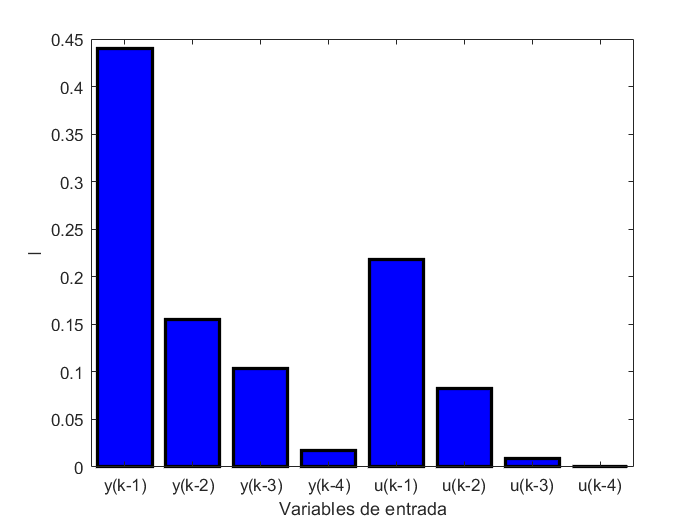
\includegraphics[width=10cm,height=7cm]{imag/P1Sensibilidad}
\caption{Índice de Sensibilidades.}
\label{f_P1Sensibilidad}
\end{figure}

La Tabla \ref{t_Error} indica el valor de la Raíz del Error Cuadrático Medio (RMSE) para los modelos con 8 y 4 regresores, y se puede notar que son muy semejantes, y por consiguiente se eselecciona el modelo más sencillo, que coincide con el número de regresores de la serie no lineal original. Recordar que RMSE se define,
\begin{equation}
RMSE=\sqrt{\frac{1}{N}\sum_{k=1}^{N}(y(k)-y_{fuzzy}(k))^2}
\label{e_RMSE}
\end{equation}
donde $N$ es la cantidad total de datos, $y(k)$ es la salida de la planta real en el instante $k$ , e $y_{fuzzy}(k)$ es la predicción realizada por el modelo difuso en el instante $k$.
% Table generated by Excel2LaTeX from sheet 'Sheet1'
\begin{table}[h!]
	\centering
	\caption{Índices de Error para el Análisis de Sensibilidades.}
	\begin{tabular}{|c|c|c|}
		\hline
		Modelo             & Variables de entrada                & RMSE                    \\ \hline
		\multirow{2}{*}{1} & $y(k-1)$,$y(k-2)$,$y(k-3)$,$y(k-4)$ & \multirow{2}{*}{0.2177} \\
		& $u(k-1)$,$u(k-2)$,$u(k-3)$,$u(k-4)$ &                         \\ \hline
		2                  & $y(k-1)$,$y(k-2)$,$u(k-1)$,$u(k-2)$ & 0.2109                  \\ \hline
	\end{tabular}
	\label{t_Error}%
\end{table}%

\item \textbf{Optimización de la estructura}:
La optimización de la estructura del modelo difuso consiste principalmente en determinar el número óptimo de reglas del modelo difuso. En este caso se definió un número máximo de 20 clusters y se entrenó el modelo para cada una de las posibles valores de clusters, utilizando como algoritmo de clustering el Fuzzy C-Means.

La Fig. \ref{f_P1reglas11} muestra el RMSE para los conjuntos de entrenamiento y prueba.  Si no importa la complejidad, el mejor modelo es aquel que
tiene menor RMSE. Sin embargo, es posible que un modelo con peor índice de
desempeño, pero menos complejo que el modelo óptimo, pueda obtener resultados
aceptables bajo un estándar de rendimiento definido preliminarmente. Por lo antes expuesto para este problema se escoge como número de clusters 5, por lo que el modelo difuso contará con 5 reglas, Fig \ref{f_Cluster}.

\begin{figure}[h!]
\centering
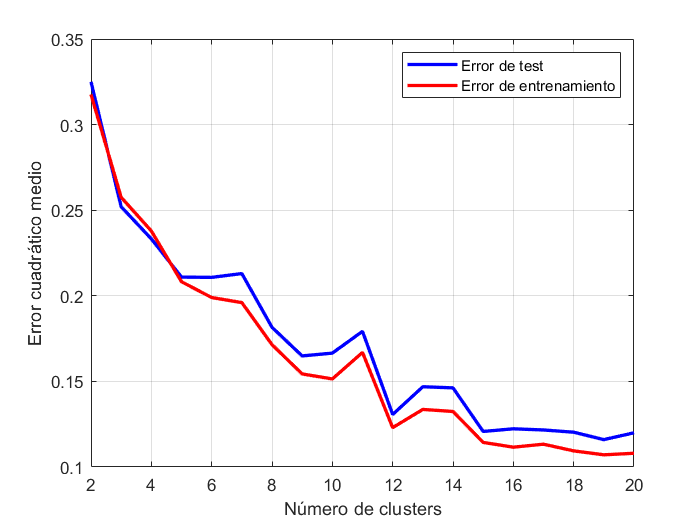
\includegraphics[width=10cm,height=7cm]{imag/P1reglas12}
\caption{Índice de Sensibilidades.}
\label{f_P1reglas11}
\end{figure}

\begin{figure}
		\centering
		\captionsetup{justification=centering}
		\subfloat[Salida]{
		 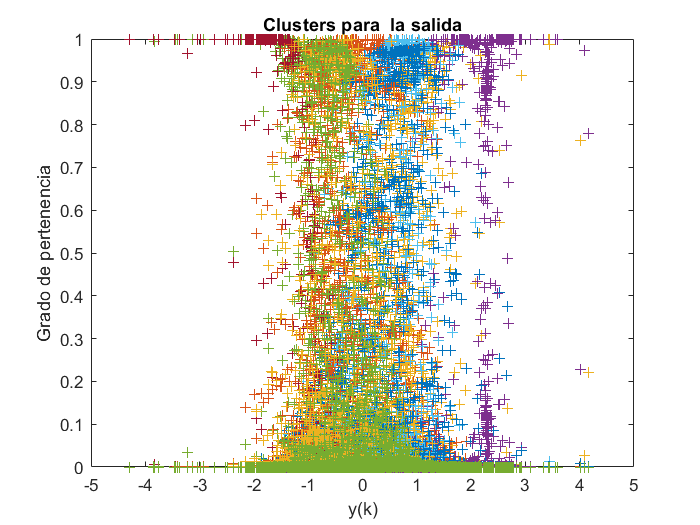
\includegraphics[width=0.5\textwidth]{imag/ClusterSalida}}\\
		\subfloat[$y(k-1)$]{
		 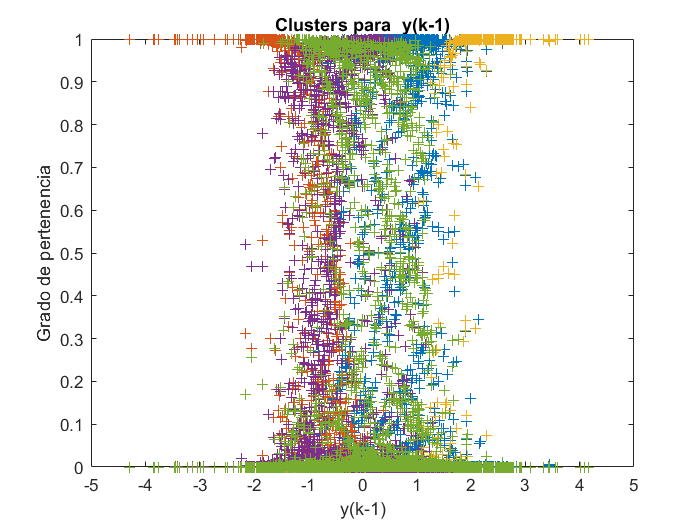
\includegraphics[width=0.5\textwidth]{imag/Clustery1}}
		\subfloat[$y(k-2)$]{
		 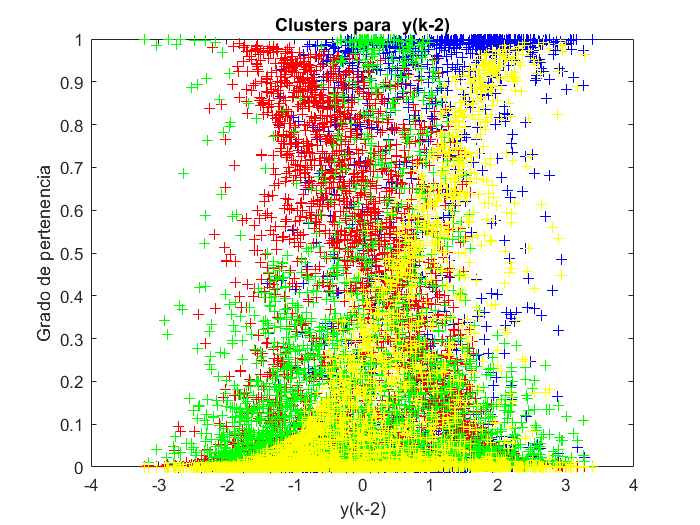
\includegraphics[width=0.5\textwidth]{imag/Clustery2}}\\
        \subfloat[$u(k-1)$]{
		 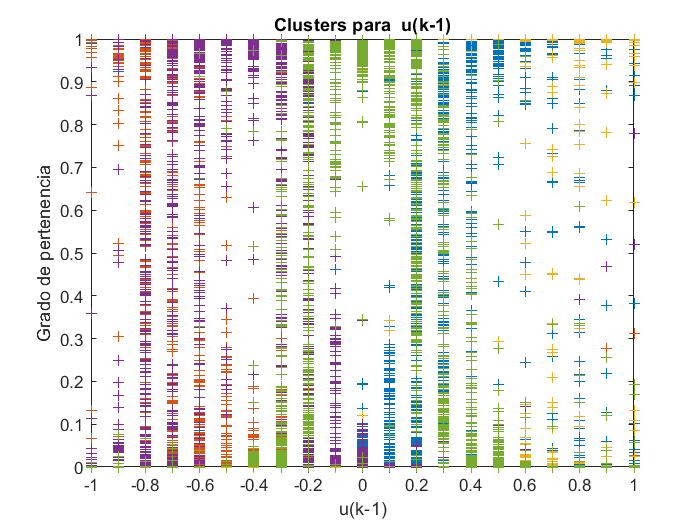
\includegraphics[width=0.5\textwidth]{imag/Clusteru1}}
		\subfloat[$u(k-2)$]{
		 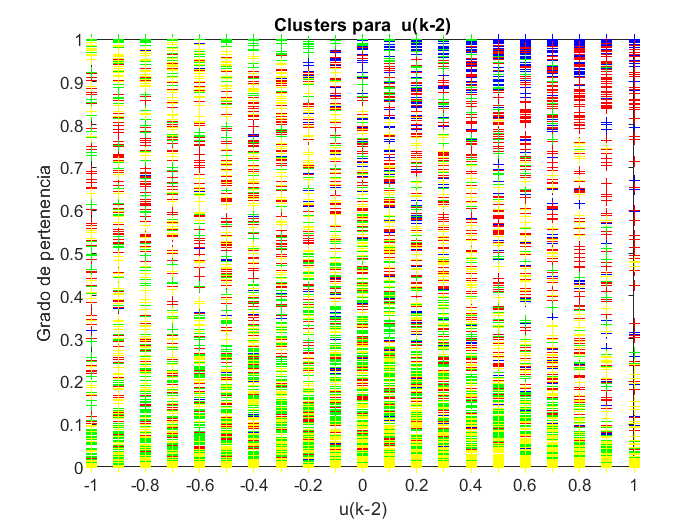
\includegraphics[width=0.5\textwidth]{imag/Clusteru2}}
		\caption{Clusters del Modelo Difuso Tipo 1.}
		\label{f_Cluster}
\end{figure}

\newpage

Una vez realizado el clustering es posible proyectar las agrupaciones en el espacio de
entrada y ajustar funciones paramétricas para describir los conjuntos difusos $MF_i^r$. En
particular, se consideraron funciones de pertenencia gaussianas dadas por

\begin{equation}
MF_r^i(z_i(k))=exp(-0.5(a_{r,i}*(z_i(k)-b_{r,i}))^2)
\label{e_Gaussiana}
\end{equation}

donde $MF_r^i(z_i(k))$ es la función de pertenencia de la i-ésima premisa $z_i(k)$ al r-ésimo
cluster, $a_{r,i}$ es el inverso de la desviación estándar de los datos ajustados por la
gaussiana, $b_{r,i}$ representa su media. Para este modelo difuso se tiene:


\begin{equation}
a=
\left(
  \begin{array}{cccc}
 1.9799	&1.4049	& 4.31509&	4.9400\\
1.8300&	1.4483	& 4.6810&	6.1218\\
2.4547	&1.8383	& 5.2820&	8.5600\\
2.0375	&1.773	& 4.5619&	4.7213\\
1.6123&	1.4681&	4.9096	&5.0399
  \end{array}
\right)
\label{e_ParA}
\end{equation}

\begin{equation}
b=
\left(
  \begin{array}{cccc}
0.6742&	0.4811&	0.4425&	0.4375\\
-1.4657&	-1.4022&	-0.7580&	-0.7632\\
2.1665&	2.1262&	0.8501&	0.86403\\
-0.43602&	-0.5047&	-0.4782&	-0.4821\\
-0.0353&	0.2984&	0.0744&	0.07290
  \end{array}
\right)
\label{e_ParB}
\end{equation}

Además del RMSE, se pueden definir el Error Porcentual Absoluto Medio (MAPE, Mean Absolute Percentage Error) y Error Absoluto Medio (MAE, Mean Absolute Error) para comprobar el modelo difuso obtenido.

\begin{equation}
MAPE=\frac{1}{N}\sum_{k=1}^{N}\frac{y(k)-y_{fuzzy}(k)}{y(k)}
\label{e_MAPE}
\end{equation}

\begin{equation}
MAE=\frac{1}{N}\sum_{k=1}^{N}|y(k)-y_{fuzzy}(k)|
\label{e_MAE}
\end{equation}


% Table generated by Excel2LaTeX from sheet 'Sheet1'
\begin{table}[htbp]
  \centering
  \caption{Índices de Error para el Modelo Difuso}
\begin{tabular}{|c|c|c|c|}
	\hline
	\multirow{2}{*}{Métricas} & \multicolumn{3}{c|}{Conjuntos}      \\ \cline{2-4}
	& Entrenamiento & Prueba & Validación \\ \hline
	RMSE                      & 0.2082        & 0.2109 & 0.1938     \\ \hline
	MAPE                      & 70.92         & 65.65  & 67.71      \\ \hline
	MAE                       & 0.1454        & 0.1505 & 0.1344     \\ \hline
\end{tabular}
  \label{t_MD}%
\end{table}%

En la Tabla \ref{t_MD} se puede ver como el RMSE se mantiene de similar para los conjuntos de prueba y validadación lo que indica la capacidad de generalización del modelo. Por su parte el índice MAPE, mide el tamaño del error (absoluto) en términos porcentuales, indicando que el error porcentual promedio del modelo se encuentra alrededor del 70\%, si bien este es un valor grande, es válido destacar que se está trabajando con una señal cuya salida se encuentra entre [-2,3]. El MAE tampoco presenta variaciones entre los diferentes conjuntos de datos. Considerando un compromiso entre complejidad y desempeño se determina que el modelo propuesto con 4 regresores y 5 reglas es suficiente.



\item \textbf{Optimización de los parámetros}: Se utiliza el algortimo de clustering difuso Fuzzy C-Means obteniéndose siguientes parámetros de los consecuentes $\theta^T=[\theta_{1,1},...,\theta_{N_r,1},...,\theta_{1,n},...,\theta_{N_r,1}]$

\begin{equation}
\theta^T=
\left(
  \begin{array}{ccccc}
 -0.1625 &	0.99755	&-0.7451	&0.8430	 &0.2983\\
0.4561&	1.1500	& -0.3126	&0.5930	& 0.1362\\
-0.2139&	0.8892&	-0.2883&	1.0148&	0.2207\\
-0.10934&	0.8182&	-0.9810&	0.6261&	0.1752\\
0.0032&	0.5939&	-0.9615&	1.0893&	0.3707
  \end{array}
\right)
\label{e_ParaModDif}
\end{equation}

\end{itemize}

\subsubsection{Predicciones a 1, 8, y 16
pasos}

Las Fig. \ref{f_SalidaModelo} muestra la salida del modelo difuso y  la estimación para 1, 8 y 16 pasos respectivamente.

\begin{figure}
		\centering
		\captionsetup{justification=centering}
		\subfloat[Salida del Modelo a 1 paso]{
		 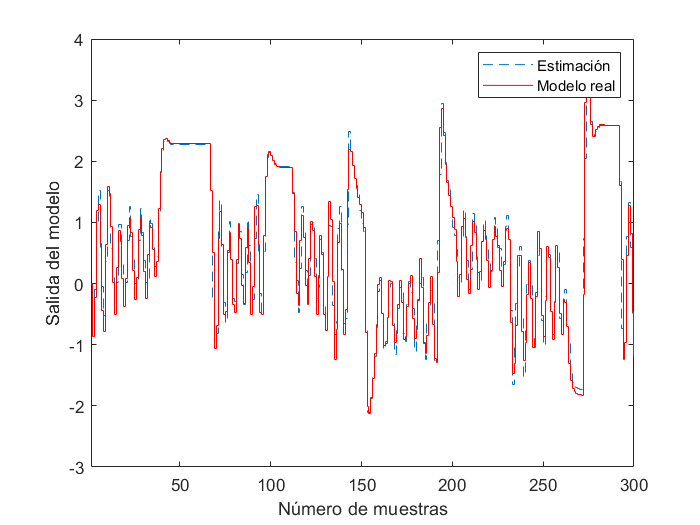
\includegraphics[width=0.5\textwidth]{imag/P1SalidaZoom}}
		%\subfloat[Salida del modelo ]{
%		 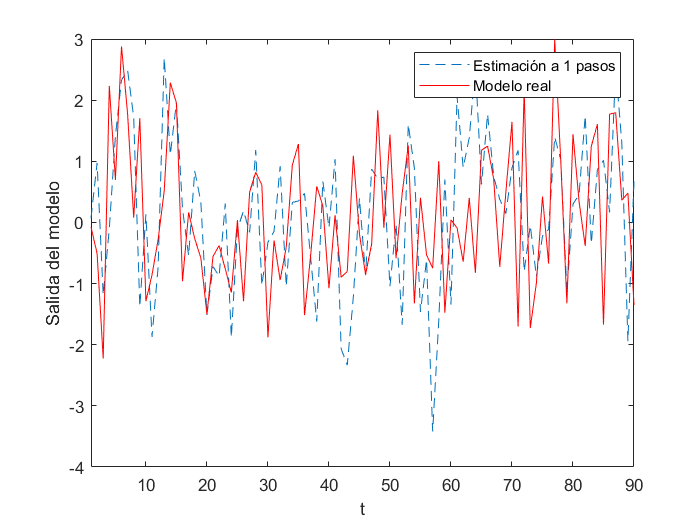
\includegraphics[width=0.5\textwidth]{imag/P1Salida_p1Zoom}}\\
        \subfloat[Salida del modelo a 8 pasos]{
		 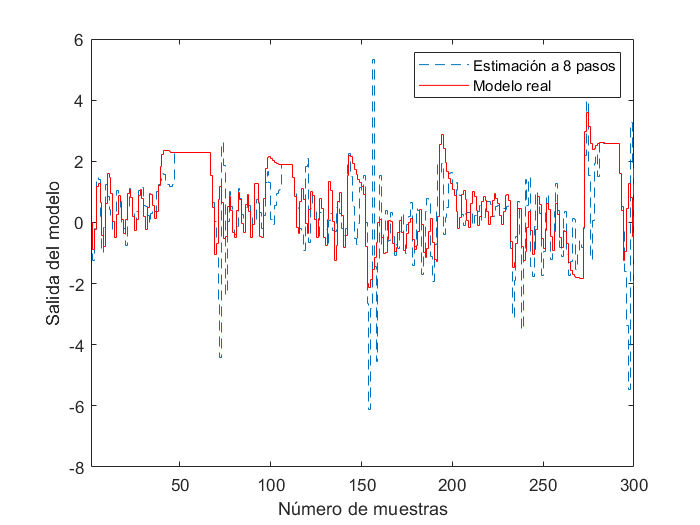
\includegraphics[width=0.5\textwidth]{imag/P1Salida_p8Zoom}}\\
		\subfloat[Salida del modelo a 16 pasos]{
		 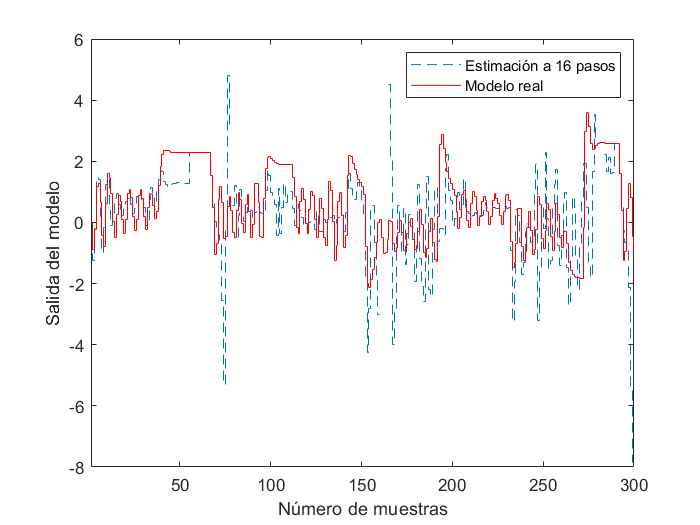
\includegraphics[width=0.5\textwidth]{imag/P1Salida_p16Zoom}}
		\caption{Respuesta del Modelo Difuso Tipo 1.}
		\label{f_SalidaModelo}
\end{figure}


En la Tabla \ref{t_MDjp} se establece una comparación entre los modelos obtenidos, como se puede comprobar a medida que aumenta el paso de la estimación el desempeño del modelo difuso se deteriora,ya que el modelo comienza a realizar estimaciones a partir de sus propias estimaciones. Sin embargo entre la estimación a 8 y 16 pasos no existen marcadas diferencias, lo cual indica que se puede utilizar el modelo obtenido para predecir a j-pasos, siempre que se tenga en cuenta que se está trabajando con estimaciones.

% Table generated by Excel2LaTeX from sheet 'Sheet1'
\begin{table}[htbp]
  \centering
  \caption{Desempeño del Modelo difuso a j-pasos}
\begin{tabular}{|c|c|c|c|}
	\hline
	\multirow{2}{*}{Métricas} & \multicolumn{3}{c|}{Modelos}                                     \\ \cline{2-4}
	& Predicción a 1 paso & Predicción a 8 pasos & Predicción a 16 pasos \\ \hline
	RMSE                      & 0.1938              & 0.6740              & 0.8653               \\ \hline
	MAPE                      & 67.71               & 147.36              & 186.32               \\ \hline
	MAE                       & 0.1344              & 0.4747              & 0.6672               \\ \hline
\end{tabular}
  \label{t_MDjp}%
\end{table}%

\subsubsection{Intervalos de predicción}

El modelo de intervalo difuso corresponde a un modelo difuso con parámetros
superiores e inferiores que contiene un porcentaje de todos los valores medidos. Se debe encontrar una
función difusa superior $\bar{f}$ y una función difusa inferior $\underline{f}$, tal que se satisfaga


\begin{equation}
\underline{f}(z_k)\leq g(z_k)\leq \bar{f}(z_k)
\label{e_InterDif}
\end{equation}

en donde $z_k\in Z$ es un conjunto de entradas, $Y={y_1,...,y_N}$ contiene los valores medidos
de la salida, y se tiene que $y_k=g(z_k),\:k=1,...,N$.

Para encontrar las funciones $\underline{f}$ y $\bar{f}$ se utilizarán dos métodos: el método
de la covarianza, y el método min-max.

El principal requerimiento al definir la banda del intervalo es que sea lo mas estrecha
posible y que contenga un cierto porcentaje de datos, llamado nivel de confianza para lo cual se definen los índices Prediction Interval Coverage
Probability (PICP) para medir el porcentaje de cobertura y el Prediction Interval Normalized
Average Width (PINAW) para medir el ancho promedio.

\begin{equation}
PICP=\frac{1}{N}\sum_{k=1}^{N}c\qquad c=\left\{
                                          \begin{array}{ll}
                                            1, & \hbox{$\hat{y}_l(k) \leq y(k) \leq \hat{y}_u(k)$} \\
                                            0, & \hbox{caso \: contrario.}
                                          \end{array}
                                        \right.
\label{e_PICP}
\end{equation}

\begin{align}
PINAW &=\frac{1}{NR}\sum_{k=1}^{N}(\hat{y}_u(k)-\hat{y}_l(k)) \qquad \\
&donde\quad R=max(y(k))-min(y(k))\nonumber
\label{e_PINAW}
\end{align}

\begin{itemize}
\item \textbf{Método de la Covarianza}:

Este método se basa en utilizar la covarianza del error entre los datos reales y la
estimación de los modelos locales del sistema difuso, de tal manera de determinar los
parámetros de las funciones difusas limitantes a partir de cada consecuencia \citep{skrjanc_confidence_2009,skrjanc_fuzzy_2011}.

\begin{equation}
Var(\hat{y}_j-h_j(Z^*)y_j)=\hat{\sigma}_j^2(1+\Psi_j^{*T}(\Psi_j\Psi_j^T)^{-1}\Psi_j^*)
\label{e_Varianza}
\end{equation}

con la que se puede definir un intervalo difuso para cada modelo local

\begin{equation}
\hat{y}^j(k)=Z^{*T}(k)\hat{\theta}_j+\alpha[Var(\hat{y}_j-h_j(Z^*)y_j)]^2
\label{e_MLocal}
\end{equation}

\begin{equation}
\hat{y}^j(k)=Z^{*T}(k)\hat{\theta}_j-\alpha[Var(\hat{y}_j-h_j(Z^*)y_j)]^2
\label{e_MLocal2}
\end{equation}

y obtener el modelo de intervalo total

\begin{equation}
\hat{y}_{u}(k)=\sum_{j=1}^{N_r}h_j(Z^*(k))*\hat{y}_u^j(k)
\label{e_ModDifusoC}
\end{equation}

\begin{equation}
\hat{y}_{l}(k)=\sum_{j=1}^{N_r}h_j(Z^*(k))*\hat{y}_l^j(k)
\label{e_ModDifusoC1}
\end{equation}

En la Tabla \ref{t_Covarianza} se muestra un análisis para tres valores de $\alpha$ diferentes, como se puede observar $\alpha=1$ da como resultado un ancho promedio porcentual del intervalo muy pequeño lo que implica un porcentaje de cobertura insuficiente para el modelo difuso, por lo cual esta opción no es válida. A medida que aumenta el valor de $\alpha$ aumenta el PICP pero también aumenta el PINAW, siendo necesario establecer un compromiso, en este problema es seleccionado el $\alpha=10$ ya que presenta para la estimación a un paso 100\% de cobertura y para las estimaciones a 8 y 16 pasos valores superiores al 75\%, aunque esto implique un aumento del PINAW. En la Fig. \ref{f_P1Covarianza} se muestra los intervalos difusos obtenidos.

En las estiamciones a j-pasos los intervalos difusos cobran una mayor importancia, pues no solo se está predidiendo un valor, sino que además se indica con cual porciento de confianza dici valor se encuentra dentro de un intervalo de tal amplitud.

\begin{figure}[h!]
		\centering
		\captionsetup{justification=centering}
		\subfloat[Salida del modelo a 1 paso.]{
		 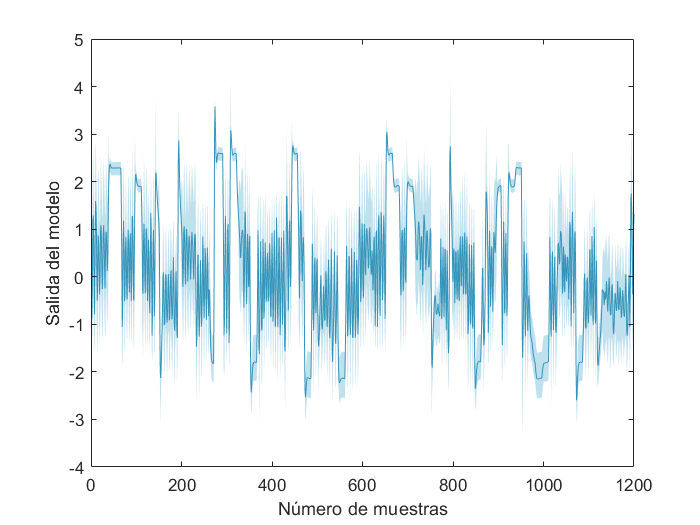
\includegraphics[width=0.5\textwidth]{imag/P1Covarianza}}
		%\subfloat[Salida del modelo ]{
%		 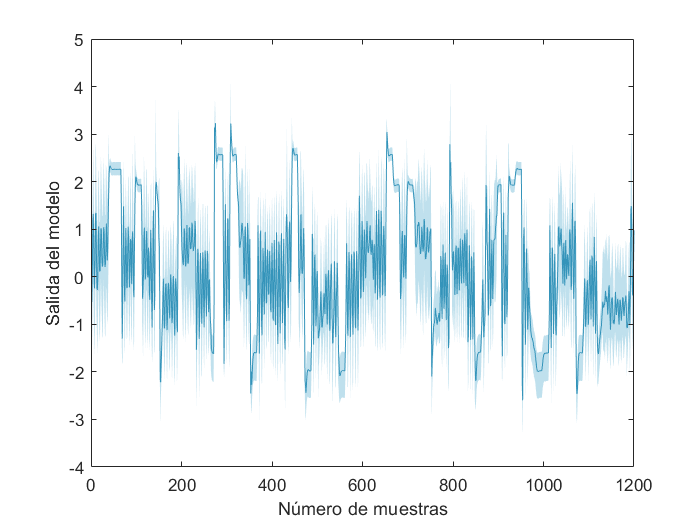
\includegraphics[width=0.5\textwidth]{imag/P1Covarianza_p1}}\\
        \subfloat[Salida del modelo a 8 pasos]{
		 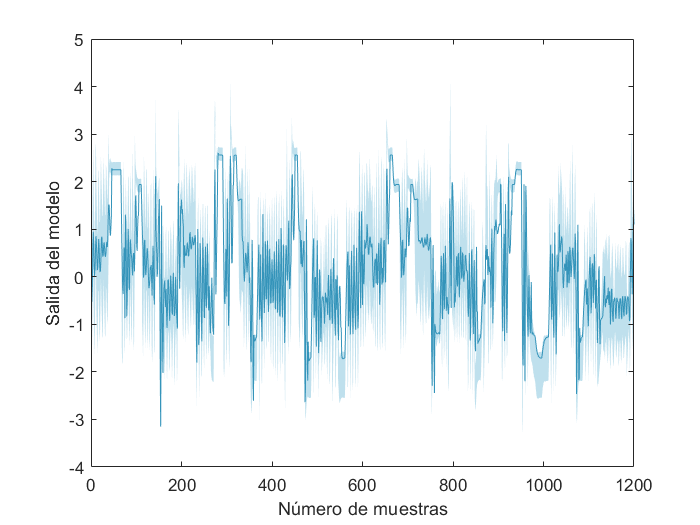
\includegraphics[width=0.5\textwidth]{imag/P1Covarianza_p8}}\\
		\subfloat[Salida del modelo a 16 pasos]{
		 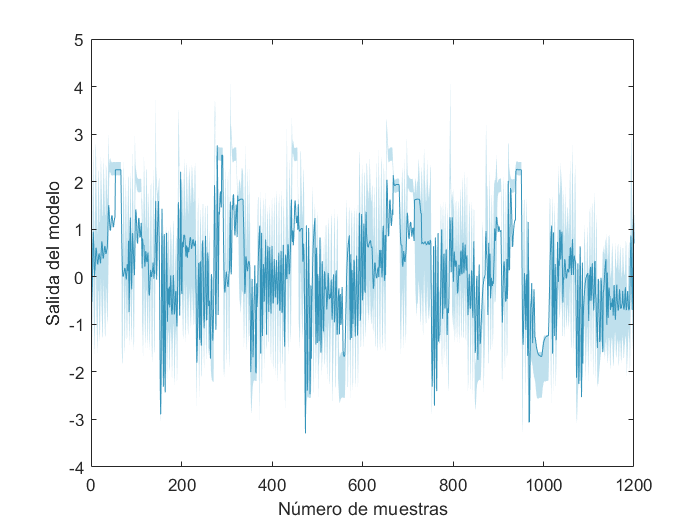
\includegraphics[width=0.5\textwidth]{imag/P1Covarianza_p16}}
		\caption{Intervalo difuso. Método de la Covarianza.}
		\label{f_P1Covarianza}
\end{figure}

% Table generated by Excel2LaTeX
\begin{table}[htbp]
  \centering
  \caption{Intervalos de predicción. Método de la Covarianza}
    \begin{tabular}{|l|r|r|r|r|r|r|r|r|r|}
    \toprule
          & \multicolumn{3}{c|}{$\alpha=1$ } & \multicolumn{3}{c|}{$\alpha=5$ } & \multicolumn{3}{c|}{$\alpha=10$ } \\
\cmidrule{2-10}    Índices & \multicolumn{1}{p{3em}|}{1 paso} & \multicolumn{1}{p{3em}|}{ 8 pasos} & \multicolumn{1}{p{3em}|}{ 16 pasos} & \multicolumn{1}{p{3em}|}{ 1 paso} & \multicolumn{1}{p{3em}|}{ 8 pasos} & \multicolumn{1}{p{3em}|}{ 16 pasos} & \multicolumn{1}{p{3em}|}{ 1 paso} & \multicolumn{1}{p{3em}|}{ 8 pasos} & \multicolumn{1}{p{3em}|}{ 16 pasos} \\
    \midrule
    PICP  & 39.5  & 14    & 9.08  & 97.5  & 63    & 47    & 100   & 86.5  & 76.25 \\
    \midrule
    PINAW & 2.76  & 2.89  & 2.97  & 13.78 & 14.448 & 14.87 & 27.55 & 28.88 & 29.74 \\
    \bottomrule
    \end{tabular}%
 \label{t_Covarianza}
\end{table}%


\newpage

\item \textbf{MinMax}:
A diferencia del anterior no se fija un porcentaje
de datos para el cual se desea el mínimo intervalo de confianza, sino que se realiza una
optimización para que se contenga la mayor cantidad de datos dentro del intervalo de
confianza y al mismo tiempo optimizando que su ancho sea el menor. Por lo que asumiendo la misma estructura de modelo obtenida anteriormente (número de reglas, número de
regresores, y parámetros de los antecedentes), se calculan los parámetros de las consecuencias de
ambos modelos ($\theta_u$,$\theta_l$ ) minimizando el máximo error absoluto de modelación mediante los siguientes
problemas de optimización

\begin{equation}
min_{\theta_u} \: max |y(k)-\sum_{j=1}^{N_r}h_j(Z^(k))*(\theta_u^j)^TZ(k)|
\label{e_MaxMin}
\end{equation}

\begin{equation}
\notag s.a \quad y(k)-\sum_{j=1}^{N_r}h_j(Z^(k))*(\theta_u^j)^TZ(k) \leq 0
\label{e_MaxMinsa}
\end{equation}

\begin{equation}
min_{\theta_l} \: max |y(k)-\sum_{j=1}^{N_r}h_j(Z^(k))*(\theta_l^j)^TZ(k)|
\label{e_MaxMin1}
\end{equation}

\begin{equation}
\notag s.a \quad y(k)-\sum_{j=1}^{N_r}h_j(Z^(k))*(\theta_l^j)^TZ(k) \geq 0
\label{e_MaxMinsa1}
\end{equation}

En la Fig. \ref{f_P1MinMax} se muestra el resultado de la aplicación del Método MinMax, para los modelos difusos obtenidos, en este caso se tiene un porcentaje de cobertura inicial de 96.92 \%, al obtenerse a partir de un algoritmo de optimización no se puede predefinir este valor; para los modelos de predicción a j-pasos el porcentaje de cobertura disminuye. El ancho promedio porcentual del intervalo que se mantiene constante para los diferentes modelos obtenidos.

\begin{figure}[t!]
		\centering
		\captionsetup{justification=centering}
		\subfloat[Salida del modelo a 1 paso.]{
		 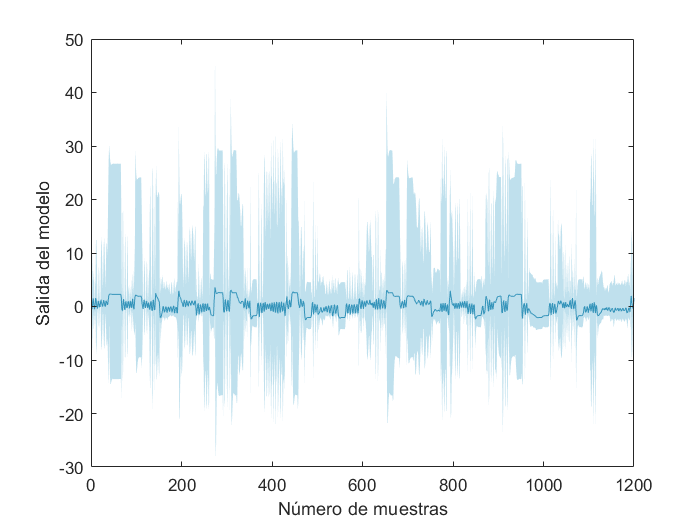
\includegraphics[width=0.5\textwidth]{imag/P1MinMax}}
		%\subfloat[Salida del modelo ]{
%		 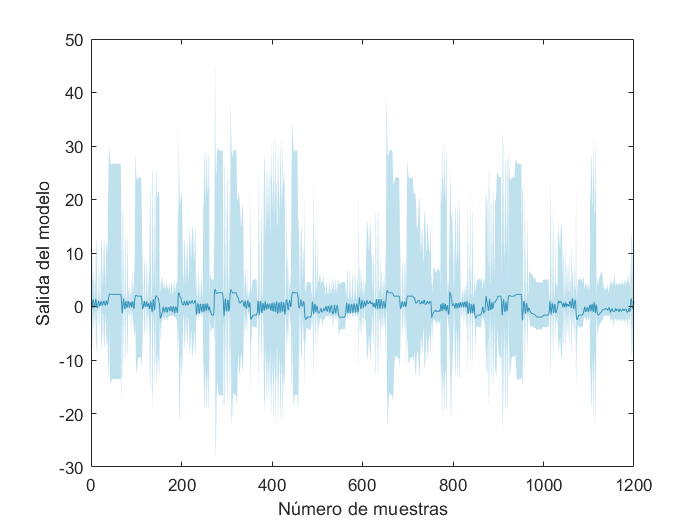
\includegraphics[width=0.5\textwidth]{imag/P1MinMax_p1}}\\
        \subfloat[Salida del modelo a 8 pasos]{
		 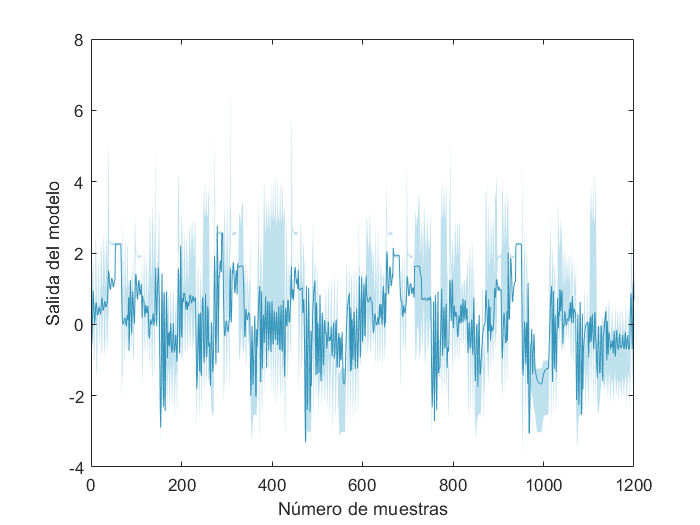
\includegraphics[width=0.5\textwidth]{imag/P1MinMax_p8}}\\
		\subfloat[Salida del modelo a 16 pasos]{
		 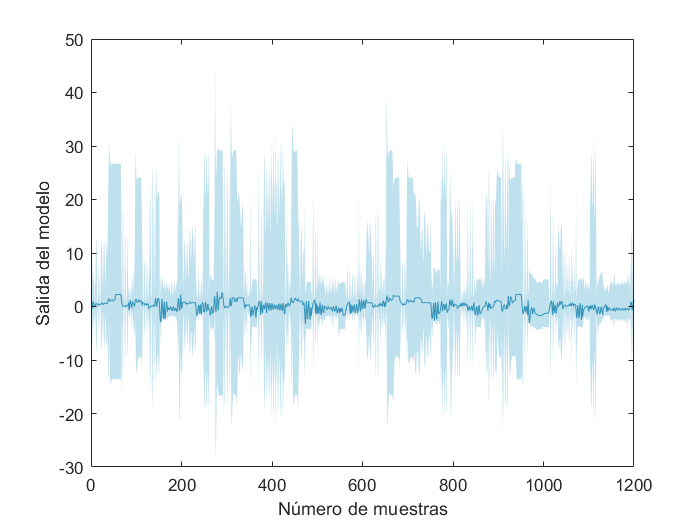
\includegraphics[width=0.5\textwidth]{imag/P1MinMax_p16}}
		\caption{Intervalo difuso. Método MinMax}
		\label{f_P1MinMax}
\end{figure}






% Table generated by Excel2LaTeX from sheet 'Sheet1'
\begin{table}[htbp]
  \centering
  \caption{Intervalos de predicción. Método MinMax}
\begin{tabular}{|c|c|c|c|}
	\hline
	\multirow{2}{*}{Métricas} & \multicolumn{3}{c|}{Modelos}                                     \\ \cline{2-4}
	& Predicción a 1 paso & Predicción a 8 paso & Predicción a 16 paso \\ \hline
	PICP                      & 92.58               & 77.25               & 69.92                \\ \hline
	PINAW                     & 30.87               & 30.71             & 33.78                \\ \hline
\end{tabular}
  \label{tab:addlabel}%
\end{table}%


\end{itemize}

Si se comparan los métodos de intervalos difusos utilizados anteriormente, se puede determinar que el método de la Covarianza con un PINAW ligeramente inferior garantiza un mejor PICP para los modelos difusos de predicción a 1, 8 y 16 pasos.

\clearpage
\newpage
\subsection{Modelo de red neuronal}

Para encontrar un buen modelo de red neuronal se propone seguir los pasos de identificación.

\begin{itemize}
	\item \textbf{Obtención de datos:} Para ello se utiliza el set de datos creado en el punto a) del problema.
	\item \textbf{Selección de datos:} Análogo a los modelos anteriores, se utilizan los datos repartido con un 55\% en el conjunto de entrenamiento, 25\% en el conjunto de prueba y 20\% en el conjunto de validación.
	\item \textbf{Definición de la estructura de la red:} Se propone una red con una capa oculta, función de activación \textit{tanh} en la salida de la capa oculta y algoritmo de aprendizaje Levenberg-Marquardt. Las variables de entradas son iguales al número de regresores (4 entradas) como muestra la Figura \ref{estred}. Por otro lado, el modelo matemático de la red, queda expresado como se muestra en la ecuacion \ref{mat_red}.
	\begin{figure}[h!]
		\centering
		 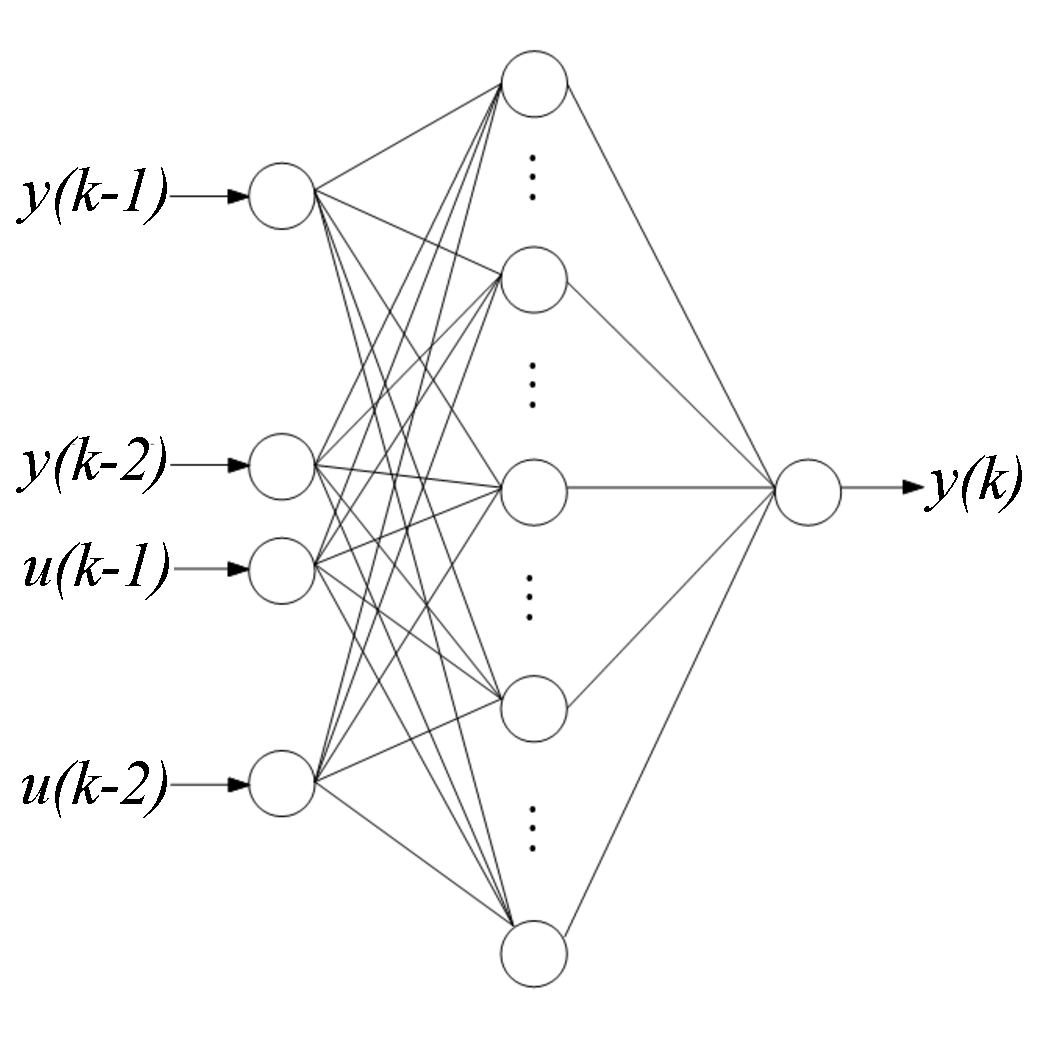
\includegraphics[width=8cm]{imag/redes/estructura.eps}
		\caption{Estructura de la red neuronal perceptrón}
		\label{estred}
	\end{figure}
	\begin{align}
	\hat{y}(k) = \sum_{i=1}^{N_h} rw_i \left( \tanh\left(\sum_{j=1}^{N_I} lw_{ji} x_j + b_i\right)\right) + c
	\label{mat_red}
	\end{align}
	
	donde, $x = [y(k-1), y(k-2), u(k-1), u(k-2)]$ es el vector de entrada, $N_h$ es el número de neuronas en la capa oculta, $N_I$ es el número de variables en la entrada, $rw_i$ es el peso que conecta la $i$-ésima neurona de la capa oculta con el nodo de salida y $lw_{ji}$ corresponde al peso que una la entrada $j$ con la $i$-ésima neurona en la capa oculta. Los sesgos de cada neuronas en la capa oculta y para el nodo de salida son $b_i$ y $c$ respectivamente.
	
	
	\item \textbf{Selección de entradas relevantes:} De los 4 regresores presente en el sistema se debe analizar cuál tiene mayor peso en el modelo. Un método para encontrar dichos regresores es mediante un análisis de sensibilidad evaluando la derivada de la salida de la red por cada premisa de nuestros datos, es decir,
	
	\begin{align}
	\xi_j = \frac{\partial \hat{y}(k)}{\partial x_j}		
	\end{align}
	Como la funcion de activacion es $tanh$ y en la salida es lineal, se tiene,
	\begin{align}
	\xi_j &= \frac{\partial \hat{y}(k)}{\partial x_j} \nonumber \\
	&= \sum_{i=1}^{Nh} rw_i \left(1 - \tanh\left(\sum_{m=1}^{N_I} lw_{mi} x_m + b_i\right)^2 \right) lw_{ji}		
	\end{align}
	
	Como se tendrá un valor de $\xi_j$ para cada dato vector de entrada, se genera un vector $\boldsymbol{\xi_j}$ del mismo largo que el número de datos de cada variable.
	
	Luego, se hace uso de un \textit{indicador} $I_j$ para cada entrada $j$ definido como,
	\begin{align}
	I_j = \mu^2 (\boldsymbol{\xi_j}) + \sigma^2(\boldsymbol{\xi_j})
	\end{align}
	donde $\mu$ es la media del vector de datos y $\sigma^2$ es la varianza para cada entrada $j$.
	
	\item \textbf{Optimización paramétrica y estructural:} Para encontrar los valores óptimos de las parámetros peso y sesgo de la red neuronal se utiliza el algoritmo de Levenberg-Marquardt backpropagation \cite{matlab_train}. Por otro lado, para encontrar el óptimo de la estructura se analiza cuantas neuronas debe tener la capa oculta. Para ello se evalúa el RMSE (Raíz del error cuadrático medio) del conjunto de prueba en la salida de la red para un número de neuronas entre $[2-41]$. Los resultados de sensibilidad para cada neurona en la capa oculta se muestran en las Figura \ref{sensi_red_1} y \ref{sensi_red_2} y el RMSE evaluado en los 3 conjuntos se muestra en la Figura \ref{RMSE_full}. Se puede ver que el mínimo RMSE para el conjunto de prueba es para $6$ neuronas y que el modelo es menos sensible  a la entrada $u(k-2)$ el cual es eliminado del entrenamiento.
	
	El entrenamiento se configura a una velocidad inicial de aprendizaje de la red de $0.05$ y un valor de épocas de 5000 con evaluación de \textit{Overfitting} de 200 épocas de validación. Es importante señalar que durante el experimento se probaron diferentes épocas de validación para cuantificar el efecto del sobre ajuste en el número óptimo de neuronas con la hipótesis de que, independiente del RMSE obtenido, el mínimo global se da con la misma cantidad de neuronas óptimas afectando solo a los mínimos locales que pudieran aparecer. En la Tabla \ref{sobreajuste} se muestran los resultados de varios experimentos demostrando la hipótesis, es más, el valor RMSE obtenido con todo los modelos es casi el mismo y solo cambia el número de neuronas, donde, $6$ demuestra ser un mínimo global y los demás un mínimo local. Por otro lado, se observo que tras varios experimentos el mejor valor RMSE del conjunto de prueba se observa cuando las épocas de validación por sobre ajuste se encuentran entre $[50-300]$, de esta manera, de aquí en adelante se utilizan 50 épocas de validación por sobre ajuste para disminuir los costos de calculo.
	\begin{table}[h!]
		\centering
		\caption{Experimento para ver la influencia del sobre ajuste.}
		\begin{tabular}{|l|l|l|}
			\hline
			Número de épocas de validación & $N_h$ óptimo & Valor RMSE \\ \hline
			1                              & 11           & 0.0025392   \\ \hline
			10                             & 7            & 0.0025384  \\ \hline
			50                             & 6            & 0.0025342  \\ \hline
			100                            & 6            & \textbf{0.0025295}  \\ \hline
			200                            & 6            & 0.0025324  \\ \hline
			500                            & 6            & 0.0025326  \\ \hline
			1000                            & 10           & 0.0025299  \\ \hline
			5000                            & 17            & 0.0025383  \\ \hline
		\end{tabular}
	\label{sobreajuste}
	\end{table}
	\newpage
	\begin{figure}[t!]
		\centering
		 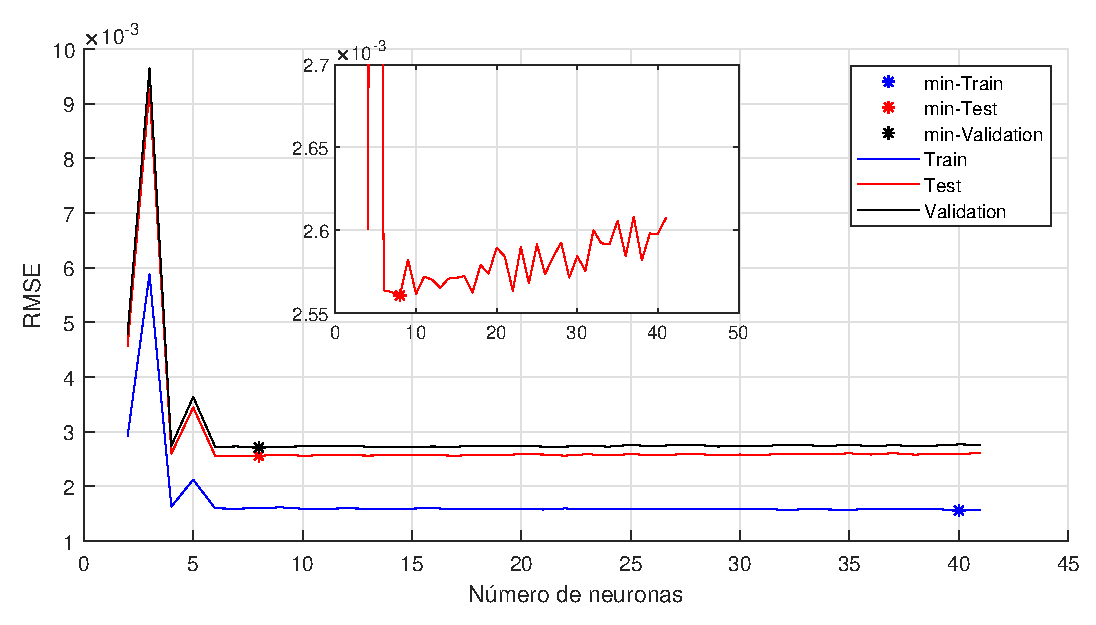
\includegraphics[width=0.8\textwidth]{imag/redes/RMSE_full.eps}
		\caption{RMSE para diferente número de neuronas.}
		\label{RMSE_full}
		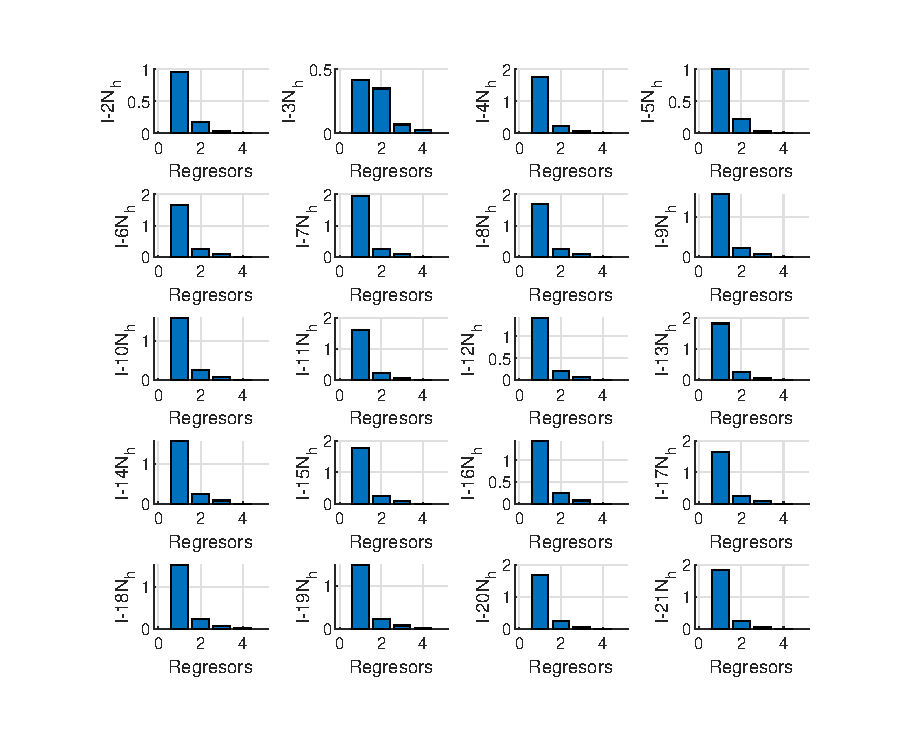
\includegraphics[width=0.8\textwidth, height=0.5\textheight]{imag/redes/sensibilidad_full_1.eps}
		\caption{Sensibilidad para un número de neuronas entre $[2-21]$ en la capa oculta.}
		\label{sensi_red_1}
	\end{figure}
	\clearpage
	\begin{figure}[t!]
		\centering
		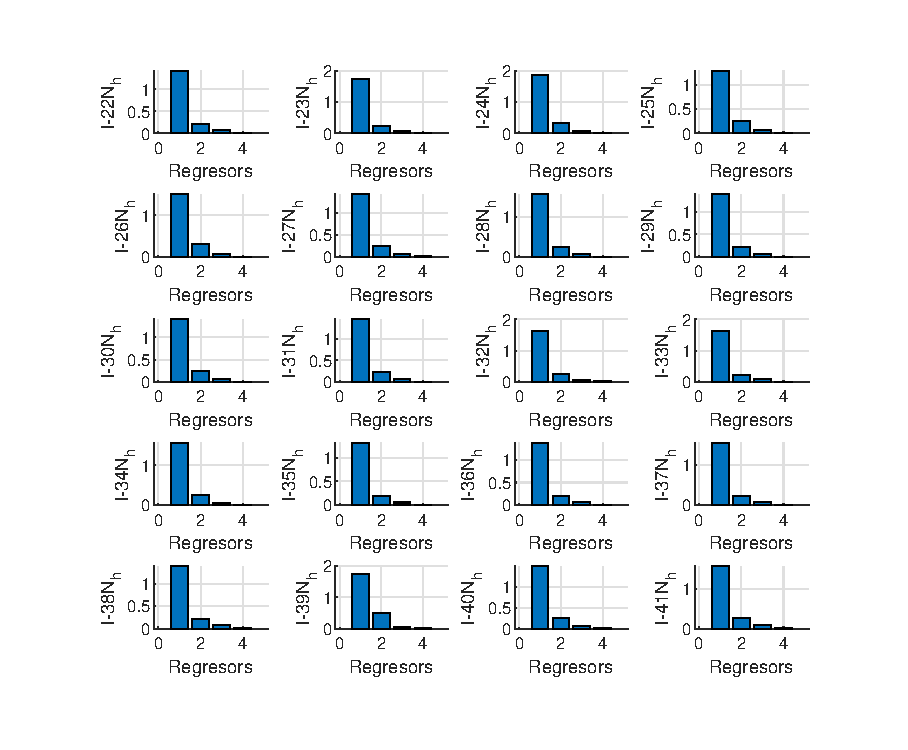
\includegraphics[width=0.8\textwidth, height=0.5\textheight]{imag/redes/sensibilidad_full_2.eps}
		\caption{Sensibilidad para un número de neuronas entre $[22-41]$ en la capa oculta.}
		\label{sensi_red_2}
	\end{figure}
	\item \textbf{Desempeño de la red definida}: Se procede a evaluar el desempeño de la red con 8 neuronas en la capa oculta utilizando las cuatro entradas y luego solo con 3, $[y(k-1), y(k-2), u(k-1)]$, para notar las diferencias.
	Los resultados se muestran en las Figuras \ref{Ind_4} hasta la \ref{hist_4} y las datos numéricos se agrupan en la Tabla \ref{tabla_red_4_3}
	
	\begin{table}[h!]
		\centering
		\captionsetup{justification=centering}
		\caption{Valores MSE para los 3 conjuntos de datos evaluados en una red con 4 entradas y otra con 3 entradas.}
		\begin{tabular}{|l|c|c|c|}
			\hline
			Número de entradas & \multicolumn{1}{l|}{MSE - Entrenamiento} & \multicolumn{1}{l|}{MSE - Prueba} & \multicolumn{1}{l|}{MSE - Validación} \\ \hline
			4                  & 0.0089                                   & 0.0097                            & 0.0084                                \\ \hline
			3                  & 0.0108                                   & 0.0118                           & 0.0108                                \\ \hline
		\end{tabular}
	\label{tabla_red_4_3}
	\end{table}

	\begin{figure}[h!]
		\centering
		\captionsetup{justification=centering}
		\subfloat[4 Entradas]{
		 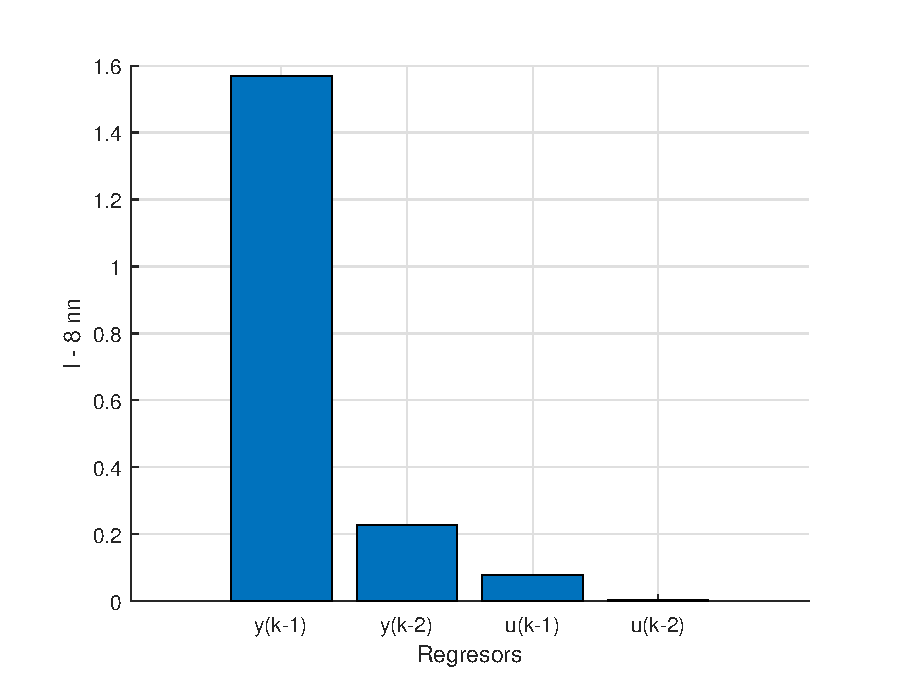
\includegraphics[width=0.5\textwidth]{imag/redes/I_4.eps}}
		\subfloat[3 Entradas]{
		 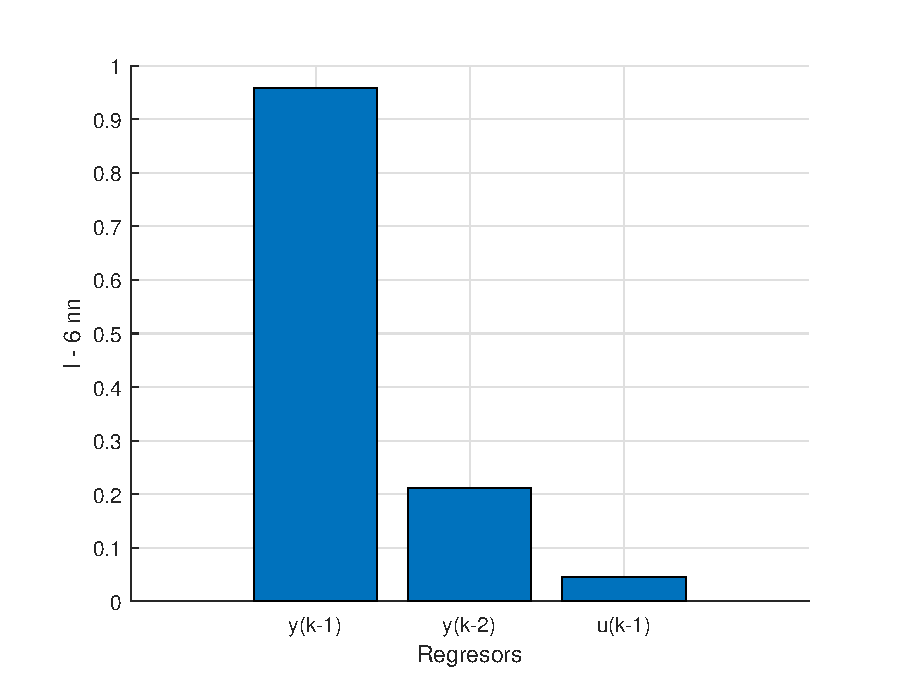
\includegraphics[width=0.5\textwidth]{imag/redes/I_3.eps}}
		\caption{Indice de sensibilidad para 4 y 3 entradas.}
		\label{Ind_4}
	\end{figure}
	Se puede notar de la Figura \ref{Ind_4} que al quitar la entrada $u(k-2)$ aumenta el indicador $I_1$ de la entrada $y(k-1)$ para compensar la falta del regresor $u(k-2)$ manteniendo casi al mismo valor las otras dos entradas. Por otro lado, no se eliminan más entradas dado que el ancho del histograma de la Figura \ref{hist_4}(b) comienza a aumentar de valor mostrando que más datos tienen errores grandes. Este error puede tener solución al utilizar un nuevo número de neuronas en la capa oculta, por lo tanto, en el siguiente ítem se procede nuevamente a encontrar el numero óptimo de neuronas con 3 entradas.
	\begin{figure}
		\centering
		\captionsetup{justification=centering}
		\subfloat[4 Entradas]{
		 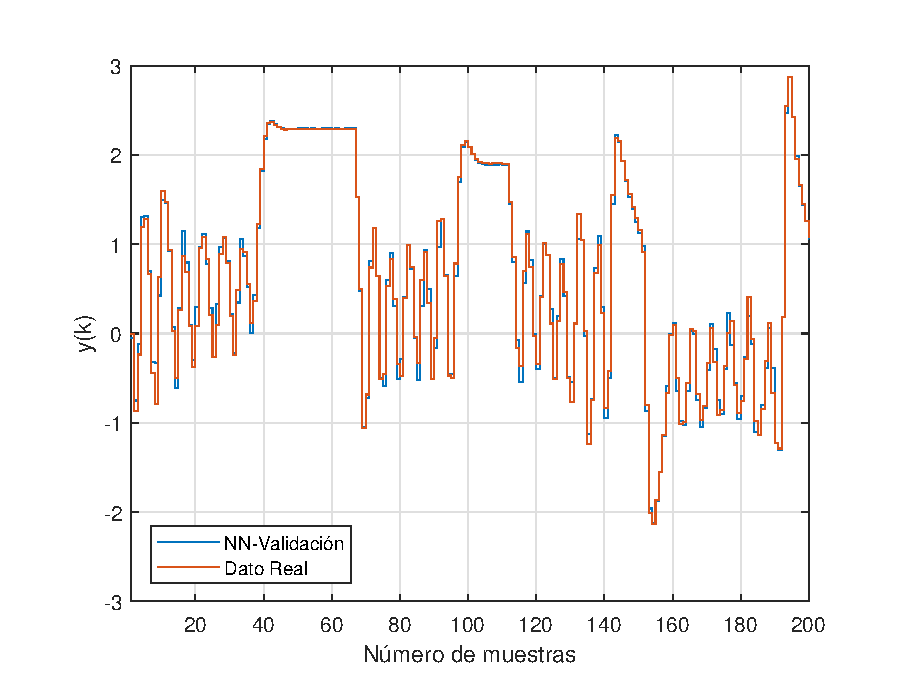
\includegraphics[width=0.5\textwidth]{imag/redes/y_red_4.eps}}
		\subfloat[3 Entradas]{
		 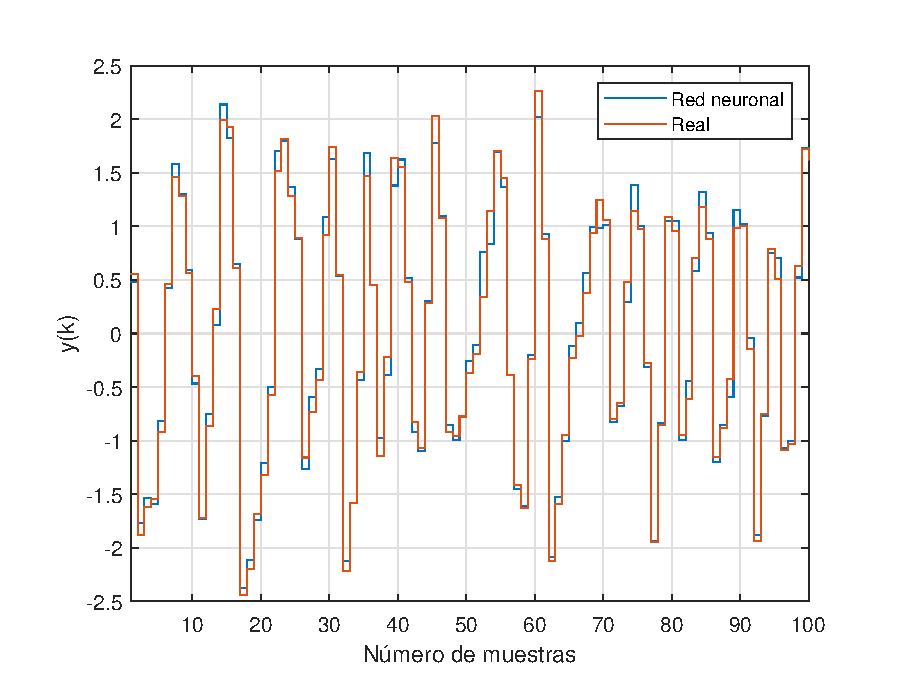
\includegraphics[width=0.5\textwidth]{imag/redes/y_red_3.eps}}
		\caption{Comparación entre la salida de la red neuronal y el valor real del conjunto de validación.}
	\end{figure}
	\begin{figure}
		\centering
		\captionsetup{justification=centering}
		\subfloat[4 Entradas]{
		 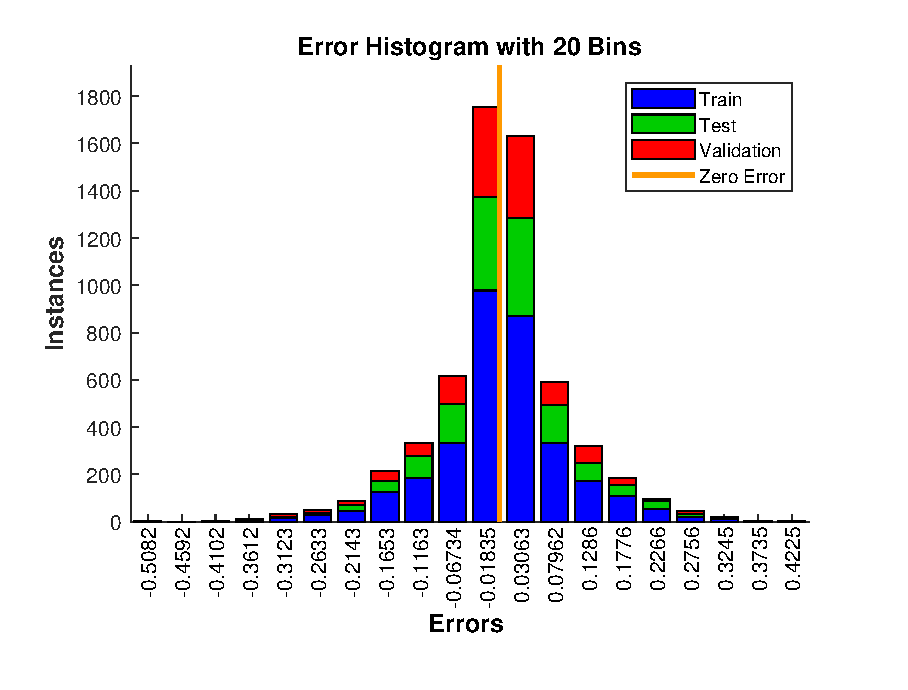
\includegraphics[width=0.5\textwidth]{imag/redes/error_4.eps}}
		\subfloat[3 Entradas]{
		 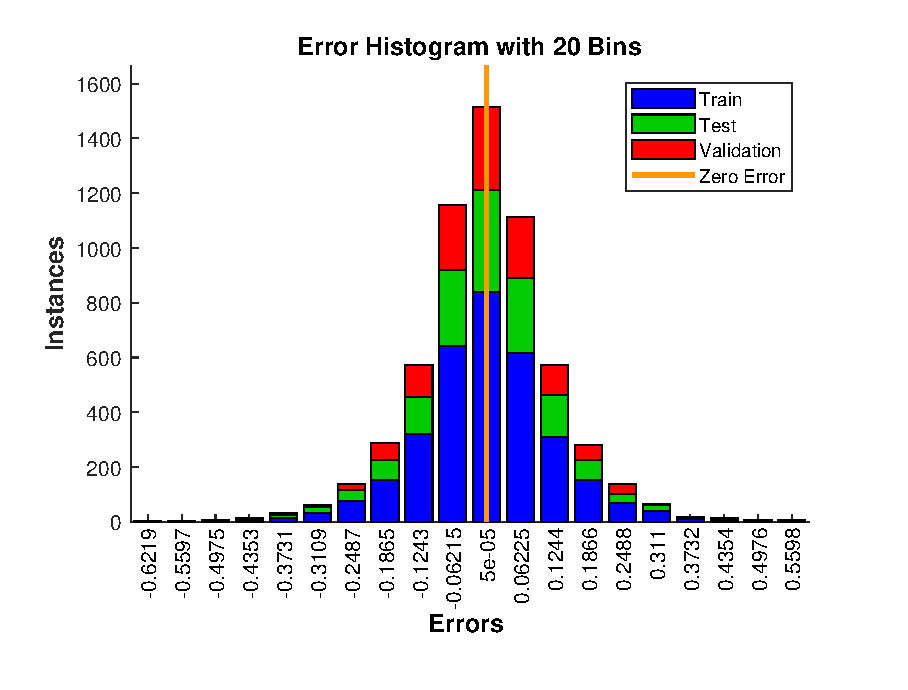
\includegraphics[width=0.5\textwidth]{imag/redes/error_3.eps}}
		\caption{Histograma del error de cada conjunto de datos.}
		\label{hist_4}
	\end{figure}

	\newpage
	\item \textbf{Optimizar estructura 2:} Se busca el número de neuronas óptimo en un rango de $[2-41]$. El resultado de la curva RMSE se muestra en la Figura \ref{rmse_3} y el análisis de sensibilidad para cada neurona en las Figuras \ref{sensi_red_1_3} y \ref{sensi_red_2_3}.

	\begin{figure}[h!]
		\centering
		\captionsetup{justification=centering}
		 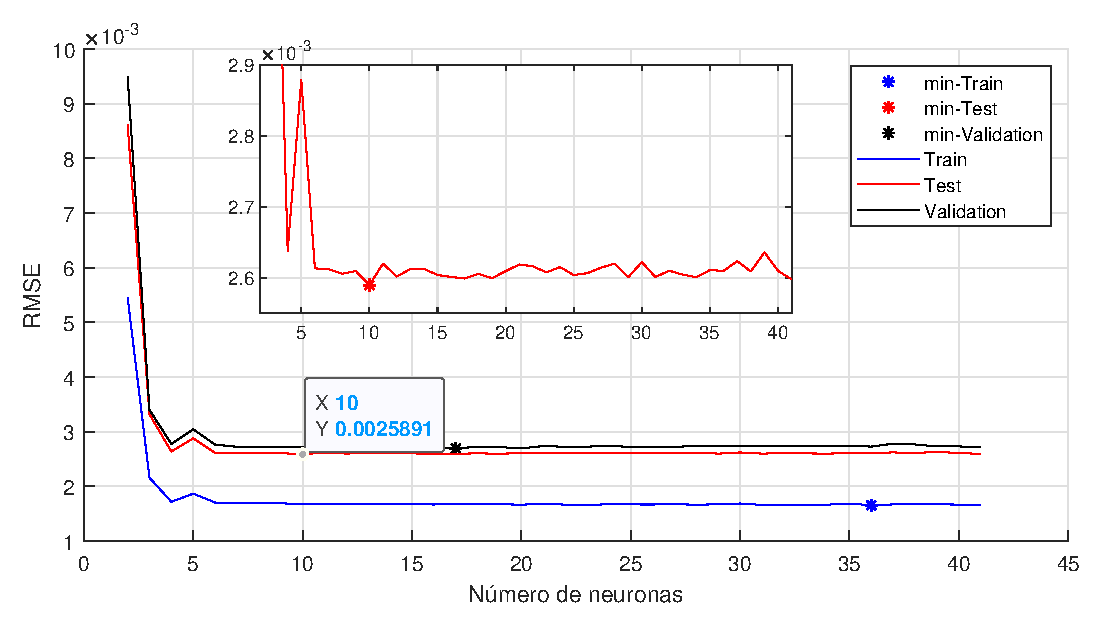
\includegraphics[width=0.8\textwidth]{imag/redes/RMSE_full_3.eps}
		\caption{RMSE para diferente número de neuronas.}
		\label{rmse_3}
	\end{figure}
	\newpage
	\clearpage
	\begin{figure}[t!]
		\centering
		\captionsetup{justification=centering}
		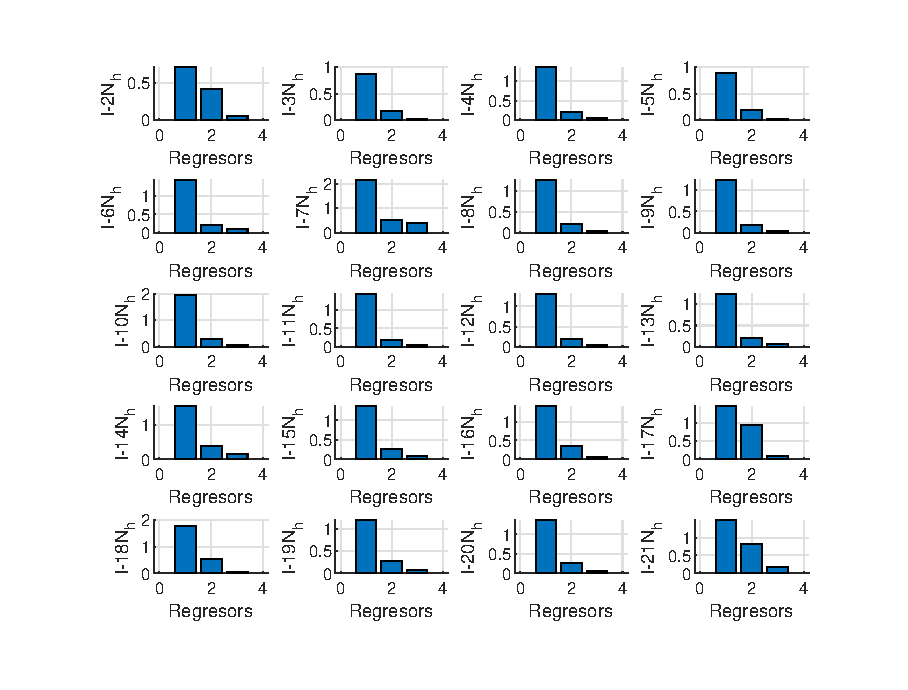
\includegraphics[width=0.8\textwidth, height=0.5\textheight]{imag/redes/sensibilidad_full_1_3.eps}
		\caption{Sensibilidad para un número de neuronas entre $[2-21]$ en la capa oculta con 3 entradas.}
		\label{sensi_red_1_3}
		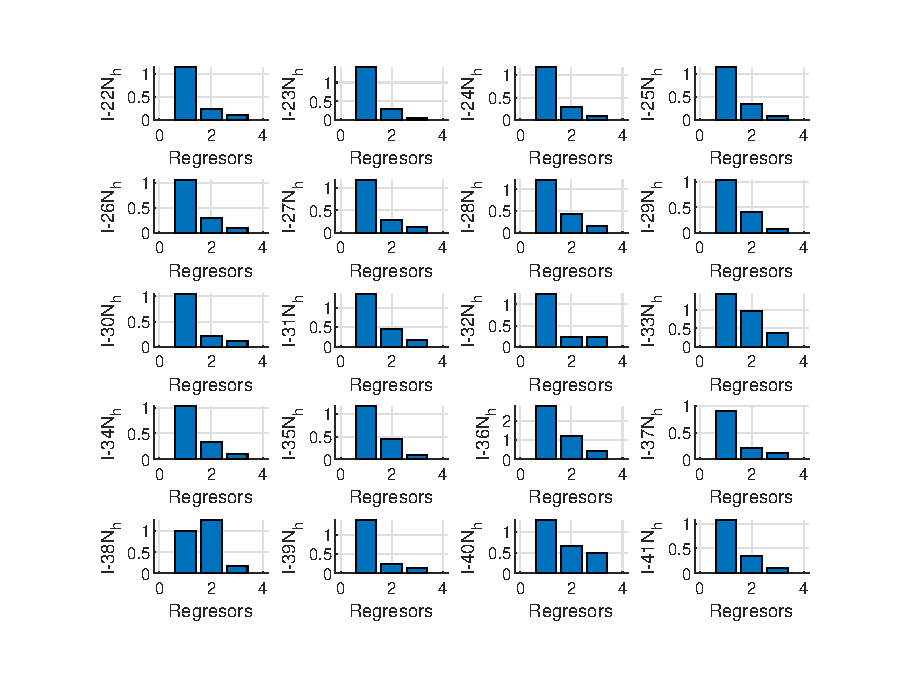
\includegraphics[width=0.8\textwidth, height=0.5\textheight]{imag/redes/sensibilidad_full_2_3.eps}
		\caption{Sensibilidad para un número de neuronas entre $[22-41]$ en la capa oculta con 3 entradas.}
		\label{sensi_red_2_3}
	\end{figure}
\end{itemize}
\newpage
\clearpage
\textbf{Validación final de la estructura:}
Para finalizar con la identificación del modelo de predicción por red neuronal, se evalúan los parámetros de la red, MAE, MAPE, RMSE, MSE reagrupados en la Tabla \ref{red_model_tabla}.

\begin{figure}[h!]
	\centering
	\captionsetup{justification=centering}
	\subfloat[RN vs datos reales]{
		 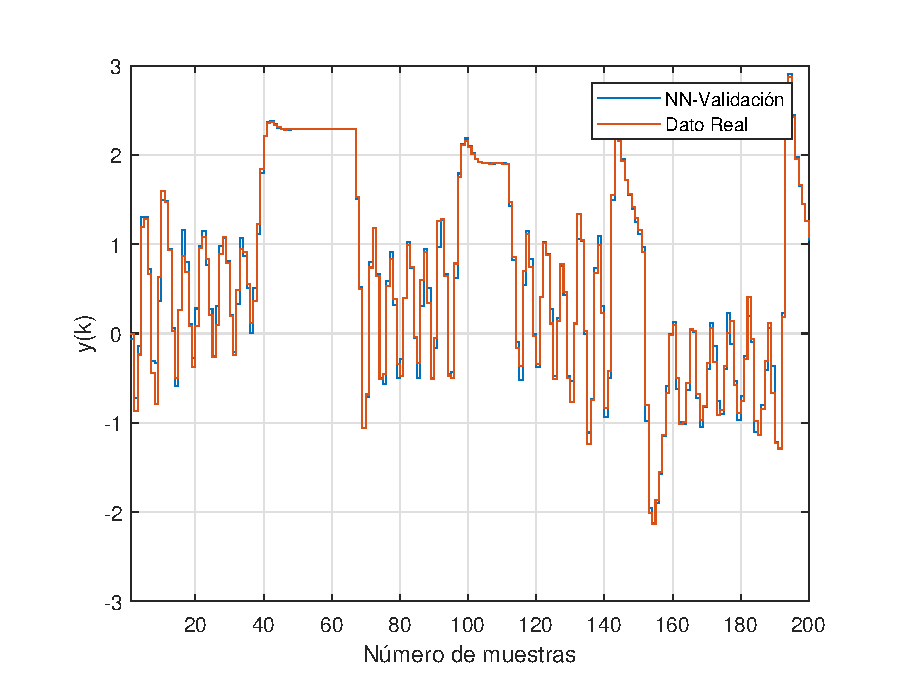
\includegraphics[width=0.5\textwidth]{imag/redes/y_red_10.eps}}
	\subfloat[Histograma del error]{
	 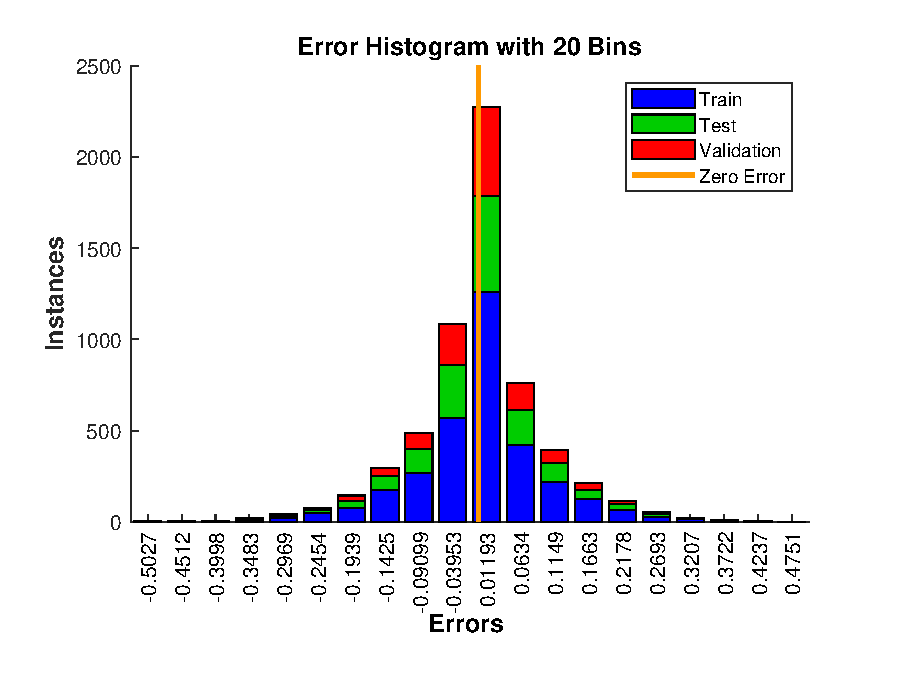
\includegraphics[width=0.5\textwidth]{imag/redes/error_10.eps}}
\caption{Resultados del modelo neuronal con 10 neuronas en la capa oculta en comparación con los datos reales.}
\end{figure}
\begin{figure}[h!]
	\centering
	\captionsetup{justification=centering}
	\subfloat[MSE de entrenamiento]{
		 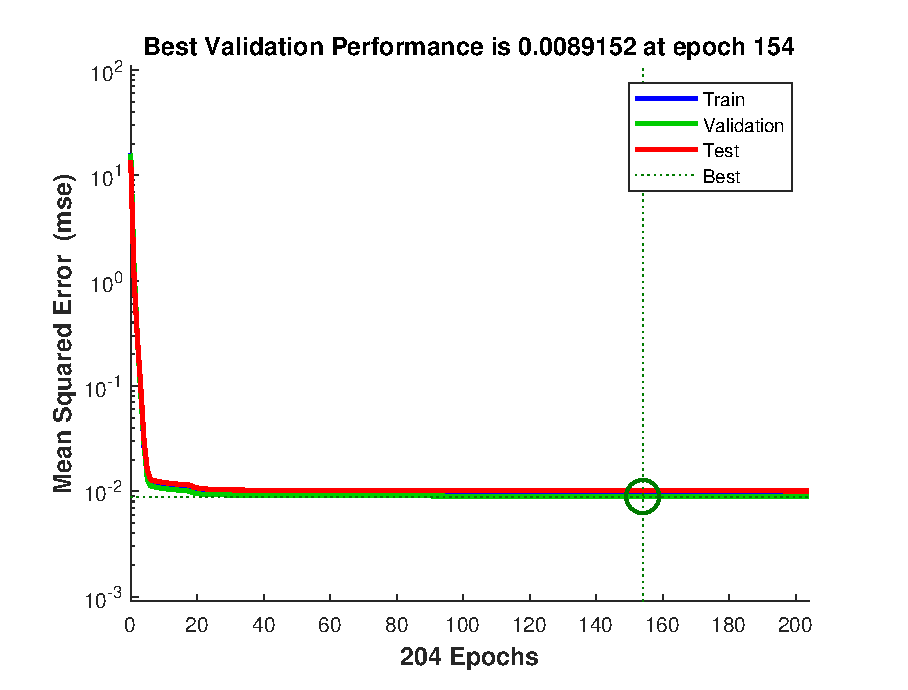
\includegraphics[width=0.5\textwidth]{imag/redes/mse_train.eps}}
	\subfloat[Regresión]{
		 \includegraphics[width=0.5\textwidth]{imag/redes/datos_target.eps}}
	\caption{Resultados de entrenamiento mostrando la regresión de cada conjunto.}
\end{figure}
\begin{table}[h!]
	\centering
	\caption{Métricas finales del modelo neuronal}
	\begin{tabular}{|l|l|l|l|}
		\hline
		Métricas & Conjunto de entrenamiento & Conjunto de prueba & Conjunto de validación \\ \hline
		RMSE     & 0.001681                  & 0.002599           & 0.002726               \\ \hline
		MSE      & 0.009324                  & 0.01013            & 0.008915               \\ \hline
		MAE      & 0.06538                   & 0.06852            & 0.06117                \\ \hline
		MAPE     & 45.25                     & 60.20              & 35.55                  \\ \hline
	\end{tabular}
\label{red_model_tabla}
\end{table}
\subsubsection{Predicciones a 1, 8, y 16
	pasos}
	Se comienza de la premisa que se conocen todos lo valores hasta $\hat{y}(k)$.
\begin{itemize}
	\item \textbf{A 1 paso:}
	Para realizar un modelo predictivo a 1 paso (un paso más y aparte del generado en si por el modelo neuronal para pasar de $(k-1)$ a $(k)$), se tiene,
	\begin{align}
	\hat{y}(k+1) &= \sum_{i=1}^{N_h} rw_i \left( \tanh\left(\sum_{m=1}^{N_I} lw_{mi} x_{m}(k + 1) + b_i\right)\right) + c
	\label{mat_red_j}
	\end{align}

	recordando la definición del vector $x$, se tiene, que $x(k+1) = [\hat{y}(k), y(k-1), u(k)]$. Existe una forma de determinar la señal de control futura $u(k)$ mediante modelo de control predictivo (MPC) \cite{norgaard_neural_2000}, sin embargo, dado que se tiene un número grande de datos y que la señal APBRS se mantiene constante por lo menos en 40 puntos por bits antes de cambiar, se dará por conocido el control $u(k)$ requerido hasta el total de datos menos $j$. Los resultados para un paso se muestran en la Figura \ref{red_1k} para todos los conjuntos de datos.
	\newpage
	\begin{figure}[t!]
		\centering
		\captionsetup{justification=centering}
		\subfloat[MSE de entrenamiento]{
			 \includegraphics[width=0.5\textwidth]{imag/redes/y_train_1k.eps}}
		\subfloat[MSE de entrenamiento]{
			 \includegraphics[width=0.5\textwidth]{imag/redes/y_test_1k.eps}}
		\newline
		\subfloat[MSE de entrenamiento]{
			 \includegraphics[width=0.5\textwidth]{imag/redes/y_val_1k.eps}}
		\subfloat[MSE de entrenamiento]{
			 \includegraphics[width=0.5\textwidth]{imag/redes/error_1k.eps}}		 
		\caption{Predicción a 1 paso con modelo neuronal.}
		\label{red_1k}
	\end{figure}
	\item \textbf{A 8 paso:}
	Para este escenario, junto al de 16 pasos, se requiere conocer entradas no conocidas. Estas entradas deben ser estimadas de los datos conocidos como muestra la Figura \ref{pred_red}, donde hasta $j=1$ se conocen los datos y para $j>=2$ se deben usar las estimaciones anteriores. Los resultados para 8 pasos se muestran en la Figura \ref{red_8k}.
	\begin{figure}[h!]
		\centering
		\captionsetup{justification=centering}
		 \includegraphics[width=0.4\textwidth]{imag/redes/pred_red.eps}
		\caption{Modelo de predicción para $j$ pasos del modelo neuronal.}
		\label{pred_red}
	\end{figure}
	\begin{figure}
	\centering
	\captionsetup{justification=centering}
	\subfloat[MSE de entrenamiento]{
		 \includegraphics[width=0.5\textwidth]{imag/redes/y_train_8k.eps}}
	\subfloat[MSE de entrenamiento]{
		 \includegraphics[width=0.5\textwidth]{imag/redes/y_test_8k.eps}}
	\newline
	\subfloat[MSE de entrenamiento]{
		 \includegraphics[width=0.5\textwidth]{imag/redes/y_val_8k.eps}}
	\subfloat[MSE de entrenamiento]{
		 \includegraphics[width=0.5\textwidth]{imag/redes/error_8k.eps}}		 
	\caption{Predicción a 8 paso con modelo neuronal.}
	\label{red_8k}
\end{figure}
\newpage
	\item \textbf{A 16 paso:} Los resultados se muestran en la Figura \ref{red_16k}.
	Reagrupando las métricas, se tiene el resultado de la Tabla \ref{tab_pred_red}.
		\begin{table}[h!]
		\centering
		\caption{Métricas de evaluación para 1, 8 y 16 pasos adelante.}
		\begin{tabular}{|l|l|l|l|}
			\hline
			 \multicolumn{4}{|c|}{\textbf{Predicción a 1 paso}}                                 \\ \hline
			Métricas & Conjunto de entrenamiento & Conjunto de prueba & Conjunto de validación \\ \hline
			RMSE     & 0.0022                    & 0.0034             & 0.0036                 \\ \hline
			MSE      & 0.0162                    & 0.0172             & 0.0157                 \\ \hline
			MAE      & 0.0917                    & 0.0948             & 0.0877                 \\ \hline
			MAPE     & 61.1581                   & 75.2533            & 37.2537                \\ \hline
			 \multicolumn{4}{|c|}{\textbf{Predicción a 8 paso}}                                 \\ \hline
			Métricas & Conjunto de entrenamiento & Conjunto de prueba & Conjunto de validación \\ \hline
			RMSE     & 0.0050                    & 0.0082             & 0.0082                 \\ \hline
			MSE      & 0.0811                    & 0.1012             & 0.0809                 \\ \hline
			MAE      & 0.2006                    & 0.2243             & 0.1900                 \\ \hline
			MAPE     & 150.8271                  & 172.2750           & 89.0900                \\ \hline
			 \multicolumn{4}{|c|}{\textbf{Predicción a 16 paso}}                                \\ \hline
			Métricas & Conjunto de entrenamiento & Conjunto de prueba & Conjunto de validación \\ \hline
			RMSE     & 0.0072                    & 0.0122             & 0.0116                 \\ \hline
			MSE      & 0.1695                    & 0.2191             & 0.1582                 \\ \hline
			MAE      & 0.2792                    & 0.3272             & 0.2621                 \\ \hline
			MAPE     & 209.8643                  & 263.4764           & 125.4239               \\ \hline
		\end{tabular}
		\label{tab_pred_red}
	\end{table}
	
		\begin{figure}[h!]
		\centering
		\captionsetup{justification=centering}
		\subfloat[MSE de entrenamiento]{
			 \includegraphics[width=0.5\textwidth]{imag/redes/y_train_16k.eps}}
		\subfloat[MSE de entrenamiento]{
			 \includegraphics[width=0.5\textwidth]{imag/redes/y_test_16k.eps}}
		\newline
		\subfloat[MSE de entrenamiento]{
			 \includegraphics[width=0.5\textwidth]{imag/redes/y_val_16k.eps}}
		\subfloat[MSE de entrenamiento]{
			 \includegraphics[width=0.5\textwidth]{imag/redes/error_16k.eps}}		 
		\caption{Predicción a 16 paso con modelo neuronal.}
		\label{red_16k}
	\end{figure}

\end{itemize}
\clearpage
\newpage
\subsubsection{Intervalo de predicción}
Para generar el intervalo de predicción en una red neuronal, se utiliza el método de la covarianza. Con este método se debe tener en cuenta algunos aspectos matemáticas que se desarrollan a continuación. Del modelo matemático de la ecuación \ref{mat_red}, es posible reescribir la ecuación separando las capas, es decir,
\begin{align}
\hat{y}(k) = \sum_{i=1}^{N_h} rw_i \tilde{Z}_i (k)  + c
\label{out_red}
\end{align}
donde $\tilde{Z}_i (k)$ es la de la $i$-ésima neurona de la capa oculta, tal que,
\begin{align}
	\tilde{Z}_i (k) &= \tanh\left(\sum_{j=1}^{N_I} lw_{ji} x_j + b_i\right) \nonumber \\
	\tilde{Z} &= LW X + B
\end{align}
Donde $\tilde{Z}$ es la matriz de todos los datos a la salida de la capa oculta, $X$ es la matriz que contiene todos los datos de la entrada, $RW$ es la matriz de los pesos internos entre la entrada y la capa oculta y $B$ es el vector de sesgo de cada neurona en la capa oculta. Luego, el método de la covarianza nos da los limites superiores $\hat{y}_u(k)$ y limite inferior $\hat{y}_l(k)$ como sigue,
\begin{align}
	\hat{y}_u(k) &= [RW \tilde{Z}^{*T}(k) + c] + \alpha \cdot \sigma_e^2 \left(1+\tilde{Z}^{*T}(k) \left(\tilde{Z} \tilde{Z}^T \right)^{-1} \tilde{Z}^{*T}(k) \right)^{1/2} \nonumber\\
	\hat{y}_l(k) &= [RW \tilde{Z}^{*T}(k) + c] - \alpha \cdot \sigma_e^2 \left(1 + \tilde{Z}^{*T}(k) \left(\tilde{Z} \tilde{Z}^T \right)^{-1} \tilde{Z}^{*T}(k) \right)^{1/2}
	\label{cov_red}
\end{align}
Donde,
\begin{itemize}
	\item $\tilde{Z}^{*T}(k)$: Es el vector/matriz del conjunto de prueba
	\item $\tilde{Z}$: Vector/matriz de los datos de entrenamiento.
	\item $RW$: Matriz de pesos que conectan la capa oculta con la capa de salida de la red.
	\item $\alpha$: Hiperparámetro para ajustar el ancho del intervalo.
	\item $\sigma_e^2$: Varianza del error en el conjunto de entrenamiento $Var(y(k) - \hat{y}(k))$.
\end{itemize}

Notar que $\tilde{Z}$ nace del conjunto de prueba, por lo tanto, para evaluar el intervalo de la varianza de validación, se deben calcular las mismas ecuaciones pero con el conjunto de validación. Por otro lado, para las predicción a $j$ pasos, se debe calcular la matriz de entrada de la red correspondiente a ese paso y calcular el valor de $\tilde{Z}$ correcto. De esta forma, se obtienen los resultados mostrados en la Figura \ref{cov_val} los resultados del conjunto de validación. Las métricas PICP y PINAW se muestran en la Tabla \ref{pinc_red}

\begin{figure}[h!]
	\centering
	\captionsetup{justification=centering}
	\subfloat[Intervalo a 1 paso]{
		 \includegraphics[width=0.5\textwidth]{imag/redes/cov_1_val.eps}}
	\subfloat[Intervalo a 8 paso]{
		 \includegraphics[width=0.5\textwidth]{imag/redes/cov_8_val.eps}} \newline
	\subfloat[Intervalo a 16 paso]{
		 \includegraphics[width=0.5\textwidth]{imag/redes/cov_16_val.eps}}
	\caption{Uso del método de covarianza para estimar el intervalo de predicción a 1, 8 y 16. Los puntos anaranjados corresponden a los datos reales de validación.}
	\label{cov_val}
\end{figure}

\begin{table}[]
	\centering
	\caption{Métricas de evaluación de intervalo para diferentes pasos con $\alpha = 5$.}
	\begin{tabular}{|l|l|l|l|}
		\hline
		\multicolumn{4}{|c|}{Conjunto de validación} \\ \hline
		PICP     & 88.0833   & 57.5859   & 48.1013   \\ \hline
		PINAW    & 4.6883    & 4.7021    & 4.7179    \\ \hline
	\end{tabular}
\label{pinc_red}
\end{table}


%\section{Problema 2}
%Para la operación óptima de las micro-redes es importante contar con modelos de predicción confiables de variables tales como: potencia solar, potencia eólica, consumo, estado de carga de las baterías, entre otras variables. Los modelos e intervalos de predicción son importantes debido a la incertidumbre asociada a la generación con energía renovable y la variabilidad del consumo local.
%
%Por tal razón, se le ha confiado a usted el proyecto de determinar modelos de predicción para la generación de energía en un sistema fotovoltaico instalado en una cierta comunidad del norte del país. La finalidad de este proyecto es la de disponer de información futura de generación fotovoltaica, para así poder gestionar el funcionamiento del resto de los elementos que componen a la micro-red.
%
%Para esto se le entregarán datos históricos de generación fotovoltaica (expresada en KW) medida en la comunidad durante el periodo septiembre-diciembre de los años 2015 y 2017. Estos datos tienen un tiempo de muestreo de 1 hora (considerar porcentajes adecuados de los datos en las fases de training, test y validación).
%
%Como usted sabe, son varias las formas que se pueden emplear para la modelación a partir de estos datos, por lo que debe seleccionar el tipo de modelo más adecuado para dicha aplicación.
%
%Se sugiere considerar los datos del año 2015 como base de entrenamiento y las mediciones del año 2017 como base de prueba y validación. Para este trabajo se le pide detallar la metodología utilizada para:
%
%\begin{enumerate}[a)]
%  \item Obtener dos modelos de predicción (a elección entre los vistos en este curso) y evaluar las predicciones a 1, 6 y 12 pasos. Comparar el desempeño de todos los modelos a partir de las métricas más apropiadas tales como RMSE, MAPE, MAE, entre otras.
%  \item Construir un intervalo de predicción para los modelos obtenidos en a), utilizando método que ud. seleccione.
%\end{enumerate}
%
%\subsection{Selección de Datos}
%Se cuenta con los datos históricos de generación fotovoltaica (expresada en KW) medida en la comunidad durante el periodo septiembre-diciembre de los años 2015 y 2017. Para la selección de los conjuntos de entrenamiento, prueba y validación se utiliza una división $[60\%,20\%,20\%]$, tomándose en este caso 2160 muestars del año 2015 para entrenamiento, que corresponde a 90 días de simulaciones, y para prueba y validación 720 muestras del año 2017, el equivalente a 30 días.

\newpage
\section{Conclusión}

En la Tabla \ref{t_Comp}, se muestran las diversas métricas de bondad de predicción para los diferentes modelos analizados en este informe (Lineal, Takagi y Sugeno y Neuronal) usando los datos de validación.

% Table generated by Excel2LaTeX from sheet 'Sheet1'
\begin{table}[htbp]
  \centering
  \caption{Comparación de los modelos propuestos}
    \begin{tabular}{|l|l|l|l|r|r|r|r|r|r|}
    \toprule
    Índices & \multicolumn{3}{c|}{Modelo Lineal} & \multicolumn{3}{c|}{Modelo Difuso Takagi Sugeno} & \multicolumn{3}{c|}{Modelo Lineal} \\
\cmidrule{2-10}          & \multicolumn{1}{p{4.055em}|}{Predicción a 1 pasos} & \multicolumn{1}{p{4.055em}|}{Predicción a 8 pasos} & \multicolumn{1}{p{4.055em}|}{Predicción a 16 pasos} & \multicolumn{1}{p{4.055em}|}{Predicción a 1 pasos} & \multicolumn{1}{p{4.055em}|}{Predicción a 8 pasos} & \multicolumn{1}{p{4.055em}|}{Predicción a 16 pasos} & \multicolumn{1}{p{4.055em}|}{Predicción a 1 pasos} & \multicolumn{1}{p{4.055em}|}{Predicción a 8 pasos} & \multicolumn{1}{p{4.055em}|}{Predicción a 16 pasos} \\
    \midrule
    RMSE  & 0.0954 & 0.0789 & 0.0964 & 0.1938 & 0.6740 & 0.8653 &       &       &  \\
    \midrule
    MAPE  & \multicolumn{1}{r|}{238.22} & \multicolumn{1}{r|}{226.60} & \multicolumn{1}{r|}{235.33} & 67.71 & 147.36 & 186.32 &       &       &  \\
    \midrule
    MAE   & 0.6020 & 0.5805 & 0.5944 & 0.1344 & 0.4747 & 0.6672 &       &       &  \\
    \bottomrule
    \end{tabular}%
  \label{t_Comp}%
\end{table}%

Un análisis para intervalos difusos se presenta con el Método de la Covarianza (común para los tres modelos utilizados) en la  Tabla \ref{t_CompCov}

% Table generated by Excel2LaTeX from sheet 'Sheet1'
\begin{table}[htbp]
  \centering
  \caption{Add caption}
    \begin{tabular}{|l|r|r|r|r|r|r|r|r|r|}
    \toprule
    Índices & \multicolumn{3}{c|}{Modelo Lineal} & \multicolumn{3}{c|}{Modelo Difuso Takagi Sugeno} & \multicolumn{3}{c|}{Modelo Lineal} \\
\cmidrule{2-10}          & \multicolumn{1}{p{4.055em}|}{Predicción a 1 pasos} & \multicolumn{1}{p{4.055em}|}{Predicción a 8 pasos} & \multicolumn{1}{p{4.055em}|}{Predicción a 16 pasos} & \multicolumn{1}{p{4.055em}|}{Predicción a 1 pasos} & \multicolumn{1}{p{4.055em}|}{Predicción a 8 pasos} & \multicolumn{1}{p{4.055em}|}{Predicción a 16 pasos} & \multicolumn{1}{p{4.055em}|}{Predicción a 1 pasos} & \multicolumn{1}{p{4.055em}|}{Predicción a 8 pasos} & \multicolumn{1}{p{4.055em}|}{Predicción a 16 pasos} \\
    \midrule
    PICP  & 52.542 & 52.797 & 52.797 & 100   & 86.5 & 76.25    &       &       &  \\
    \midrule
    PINAW & 18.6992   & 18.4244   & 18.7348   & 27.55  & 28.88 & 29.74  &       &       &  \\
    \bottomrule
    \end{tabular}%
  \label{t_CompCov}%
\end{table}%


				



\newpage
\bibliographystyle{IEEEtran}
\bibliography{biblio}
\end{document} 